\section{Image \& layer characterization}
\label{sec:redundant_layers}

%\nancomment{This section provides the basic charact}
In this section, we present comprehensive characterization of Docker images and
layers.  We analyze and present the highlights of dataset stored by Docker Hub
registry.  We also provide useful insights (parameters or metrics)
for the developers to better
understand the file systems used by Docker container. 

This analysis is particularly useful as no prior work exists on union file
systems~\cite{xxx} and dataset used and created exclusively for Docker,
which are different from either analysis on EX4 linux file system~\cite{xxx} or
Windows file system~\cite{xxx}. 


\subsection{Layer and image size}
\nancomment{cache parameters, bigger image/layer overhead for runtime}
\begin{figure}[!t]
	\subfigure[CDF of layer size]{\label{fig_layer_size}
		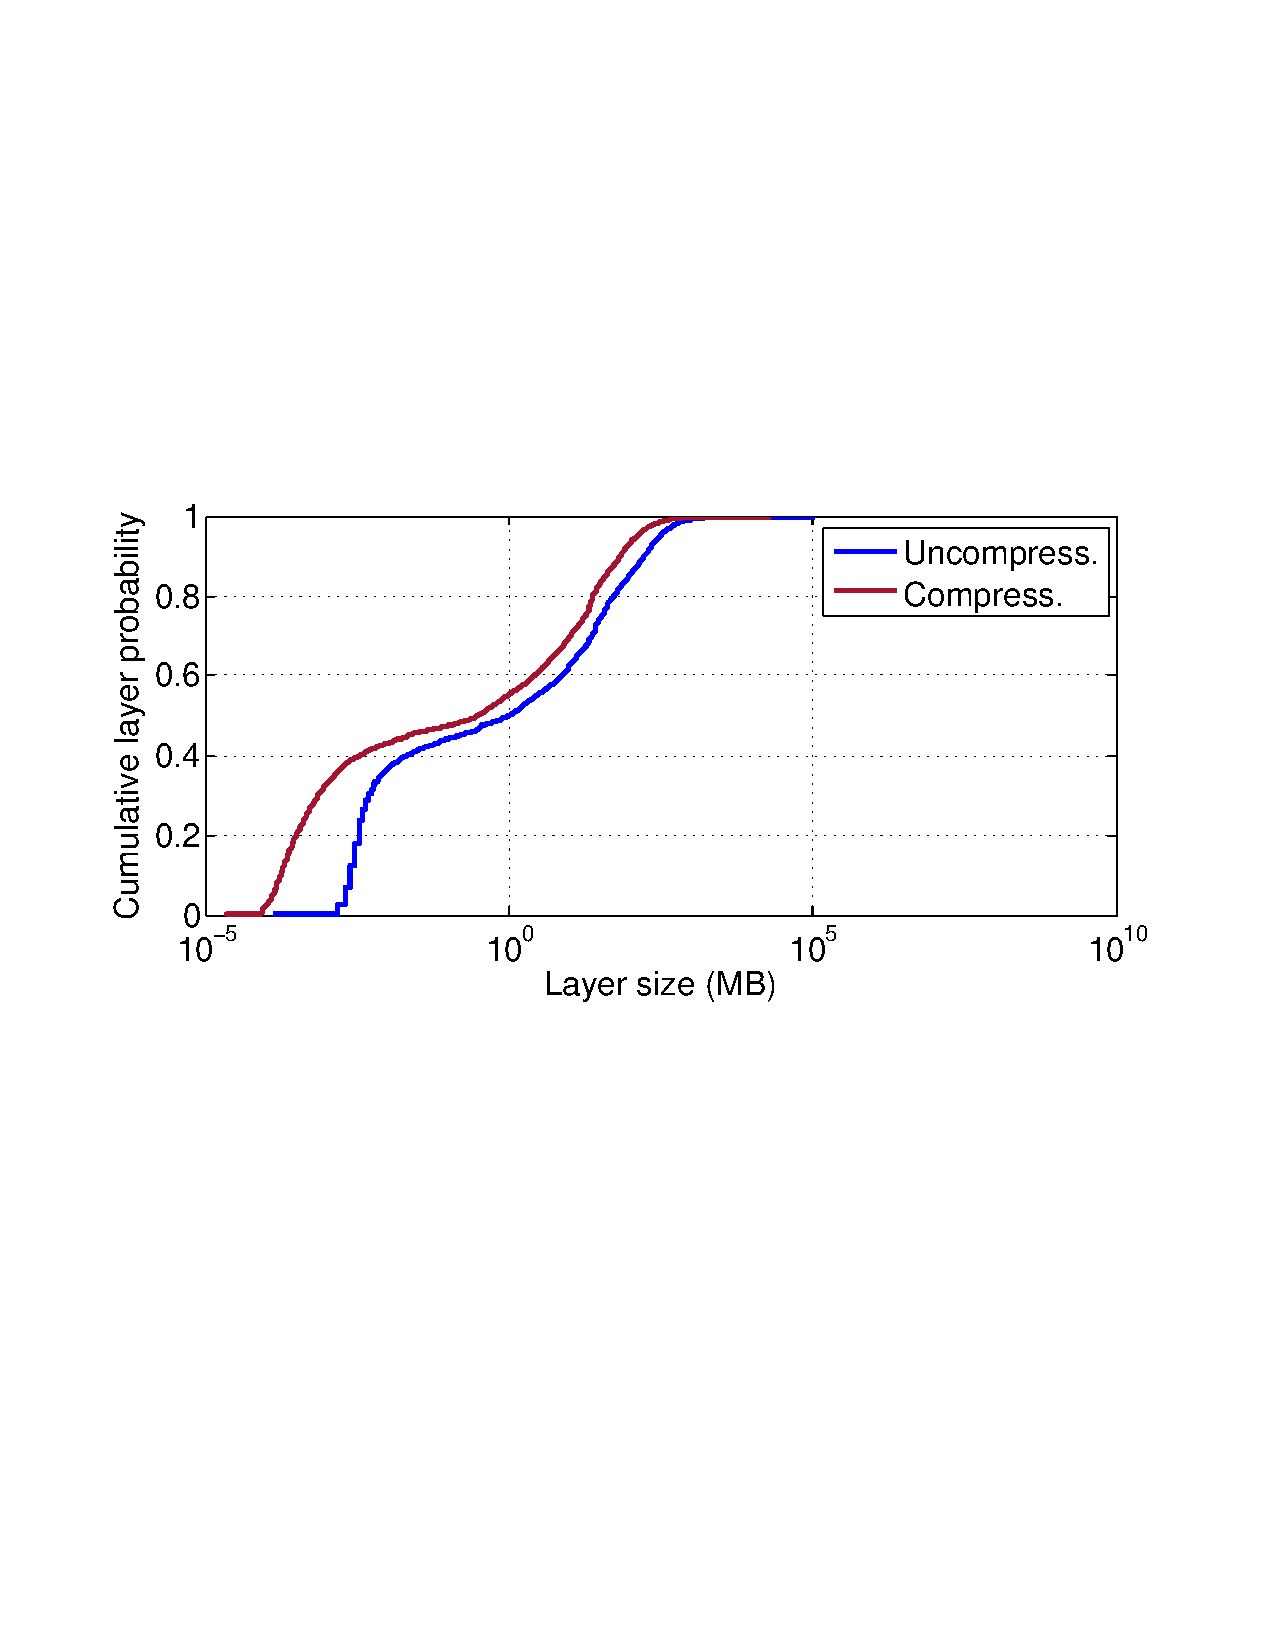
\includegraphics[width=0.4\textwidth]{graphs/layer-size-cdf.pdf}
	}
	\centering
	\subfigure[CDF of image size]{\label{fig_image_size}
		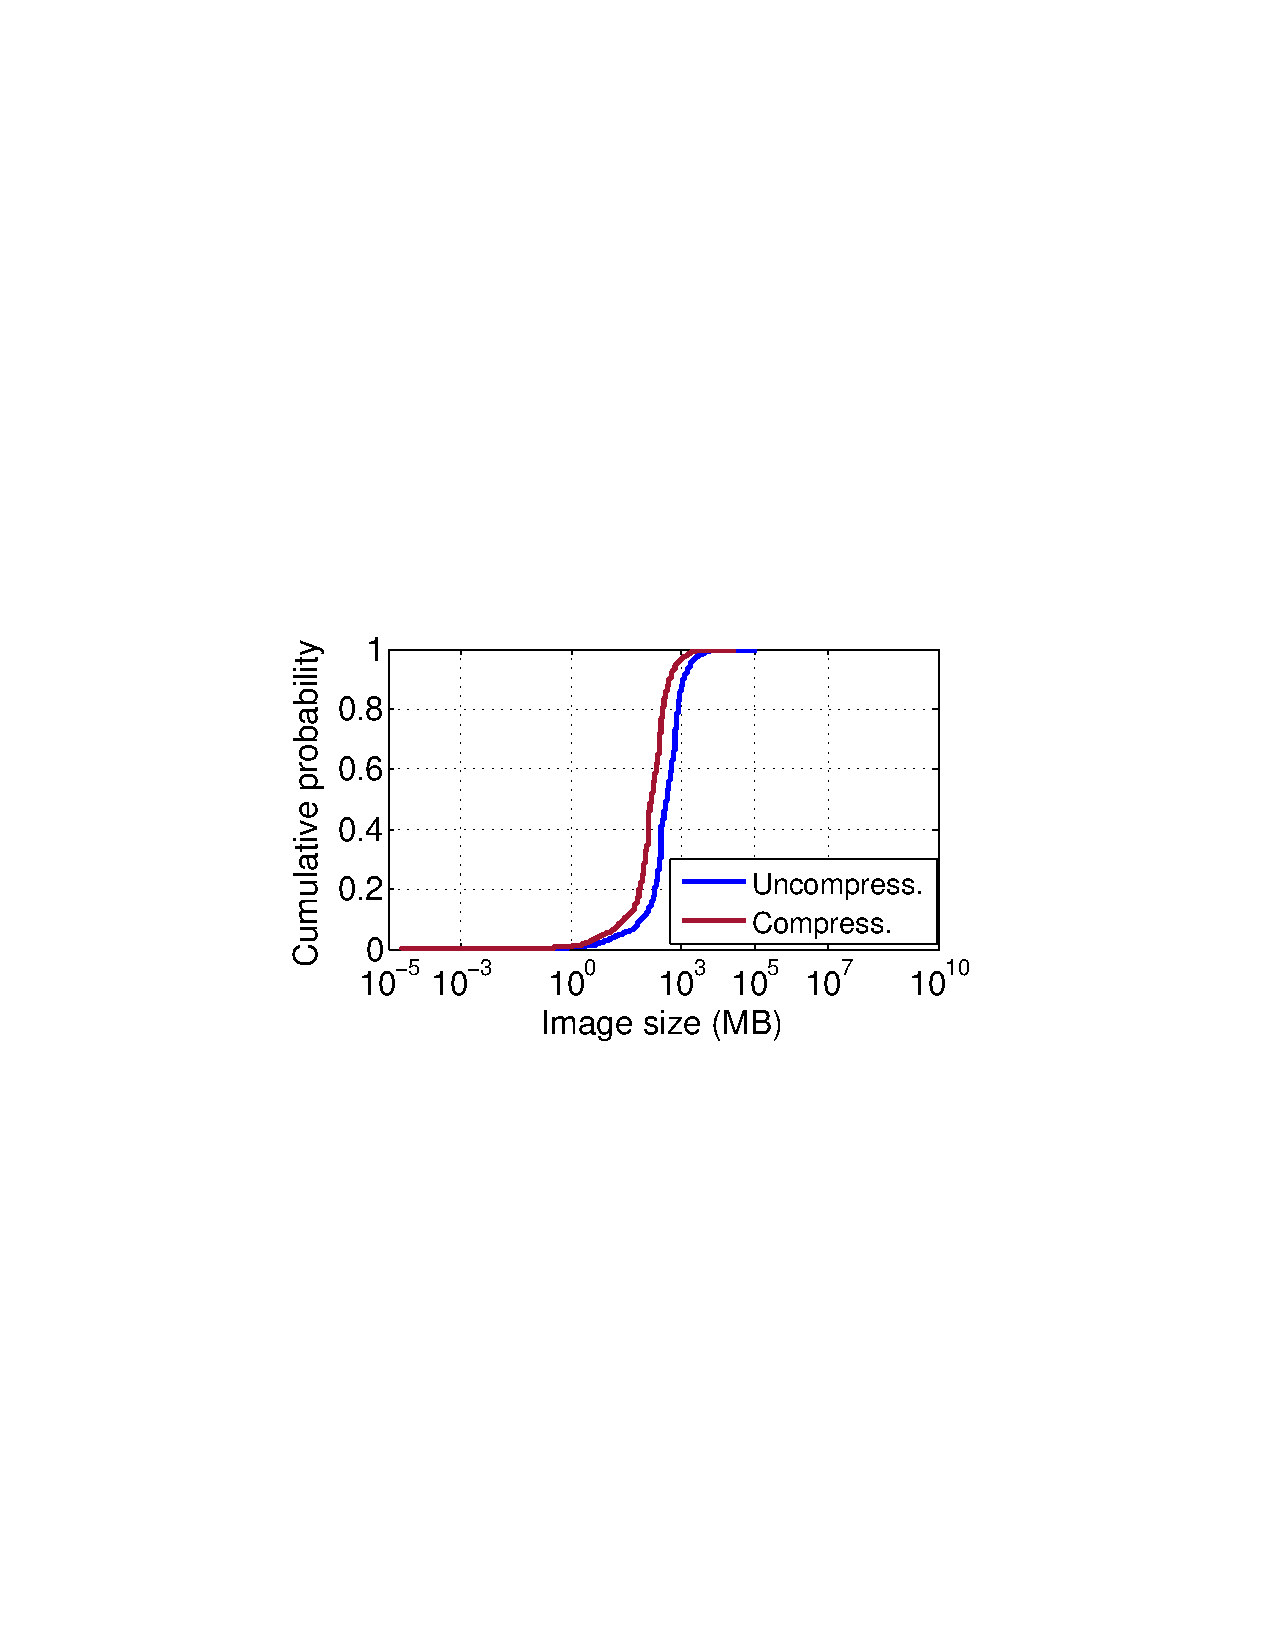
\includegraphics[width=0.4\textwidth]{graphs/image-size-cdf.pdf}%
	}

	\caption{Image/layer size distribution}
	\label{fig:image-layer-size}
\end{figure}

Recall that container image consists of multiple layers and each of these layer
is stored in Docker registry.  In figure~\ref{fig_layer_size} we show the layer
size distribution. We find that around 50\% of the layers are 1~MB in size and
90~\% of layers are less than 100~MB. This finding is particularly useful for
the Docker registry designers as it shows that selective or popular layers can
be cached in memory at the registry side.

\acomment{Where is layers analysis when you say similarly? I wrote above
para.. see for consistency.}
%Conatiner image size determines the runtime of container if it is not already
%cached locally. 
Similar to layers, we measure compressed image size (CIS), \ie the sum of the
sizes of the compressed image layers, and the sum of the sizes of files
contained in the image (FIS). Figure~\ref{fig_image_size}
and~\ref{fig_image_size_mb} show the image size distributions at a coarse GB
resolution and a finer resolution only covering images smaller than 1.5 GB.
\acomment{Could not locate the figures you are talking about. I see two figures
layers size and image size.}

Figure~\ref{fig_image_size} shows that the majority of uncompressed images in
Docker Hub are small which aligns with the Docker philosophy to package
software and distribute software in containers but include only its necessary
dependencies.

\subsection{Compression ratio}
\begin{figure}
	\centering
	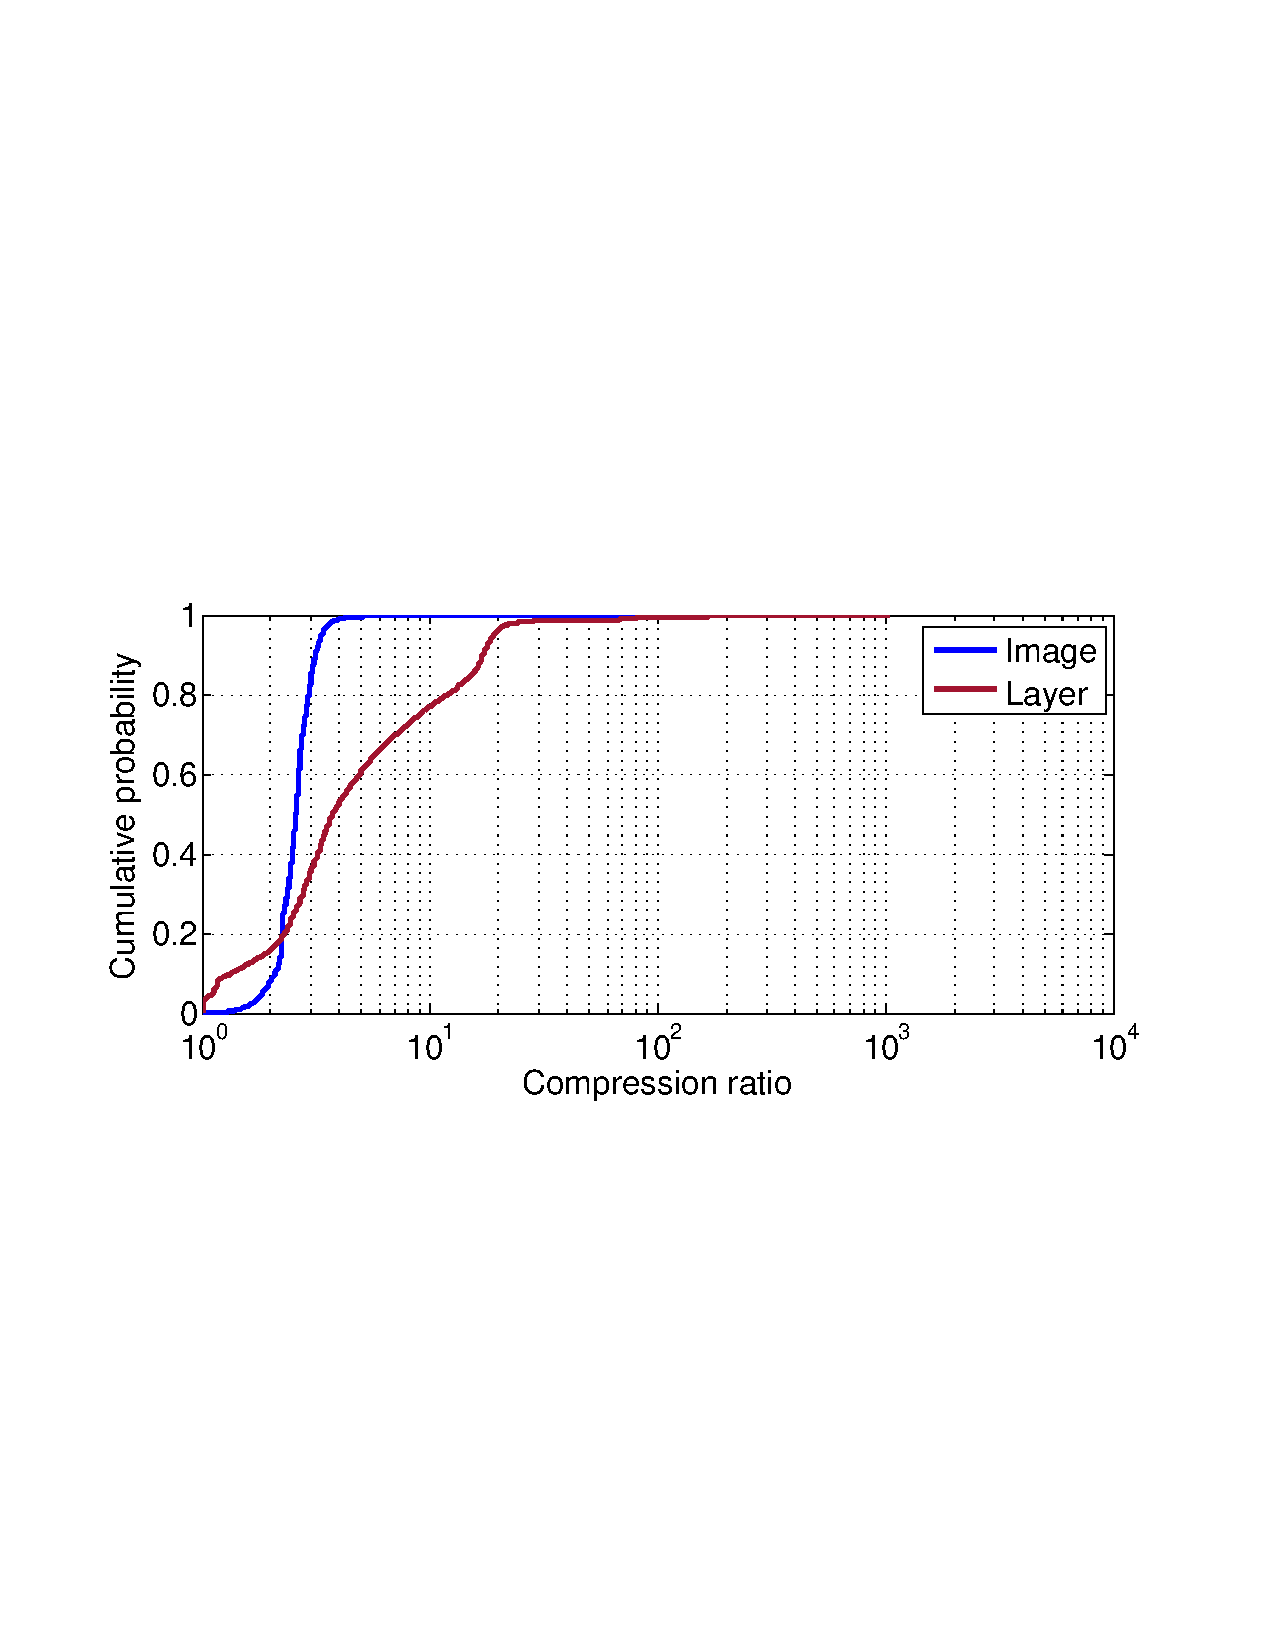
\includegraphics[width=0.4\textwidth]{graphs/compress-ratio-cdf.pdf}
	\caption{CDF of compression ratio.
	}
	\label{fig:compress-ratio}
\end{figure}

\begin{figure}[!t]
	\centering
	\subfigure[Image compression ratio]{\label{fig_hist_image}
		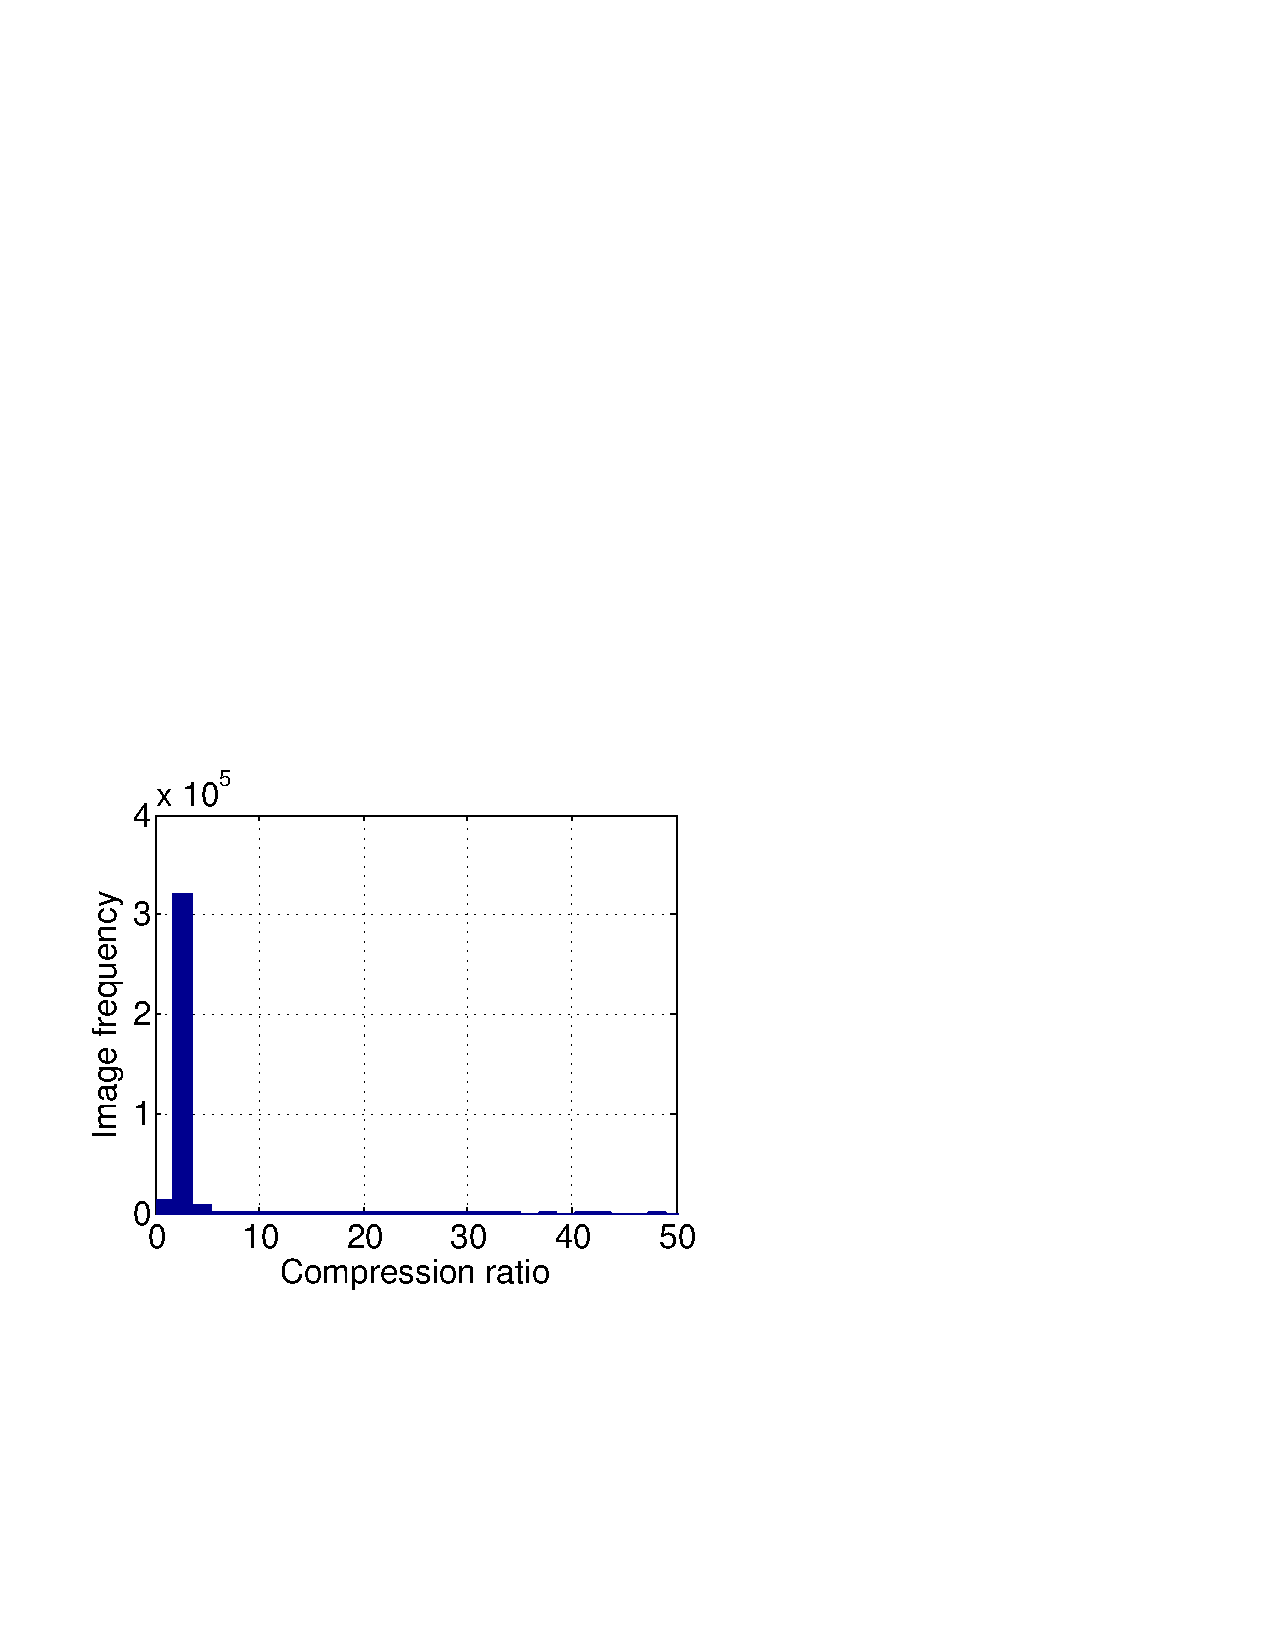
\includegraphics[width=0.215\textwidth]{graphs/image-compress-ratio-pdf.pdf}%
	}
	\subfigure[Layer compression ratio]{\label{fig_hist_layer}
		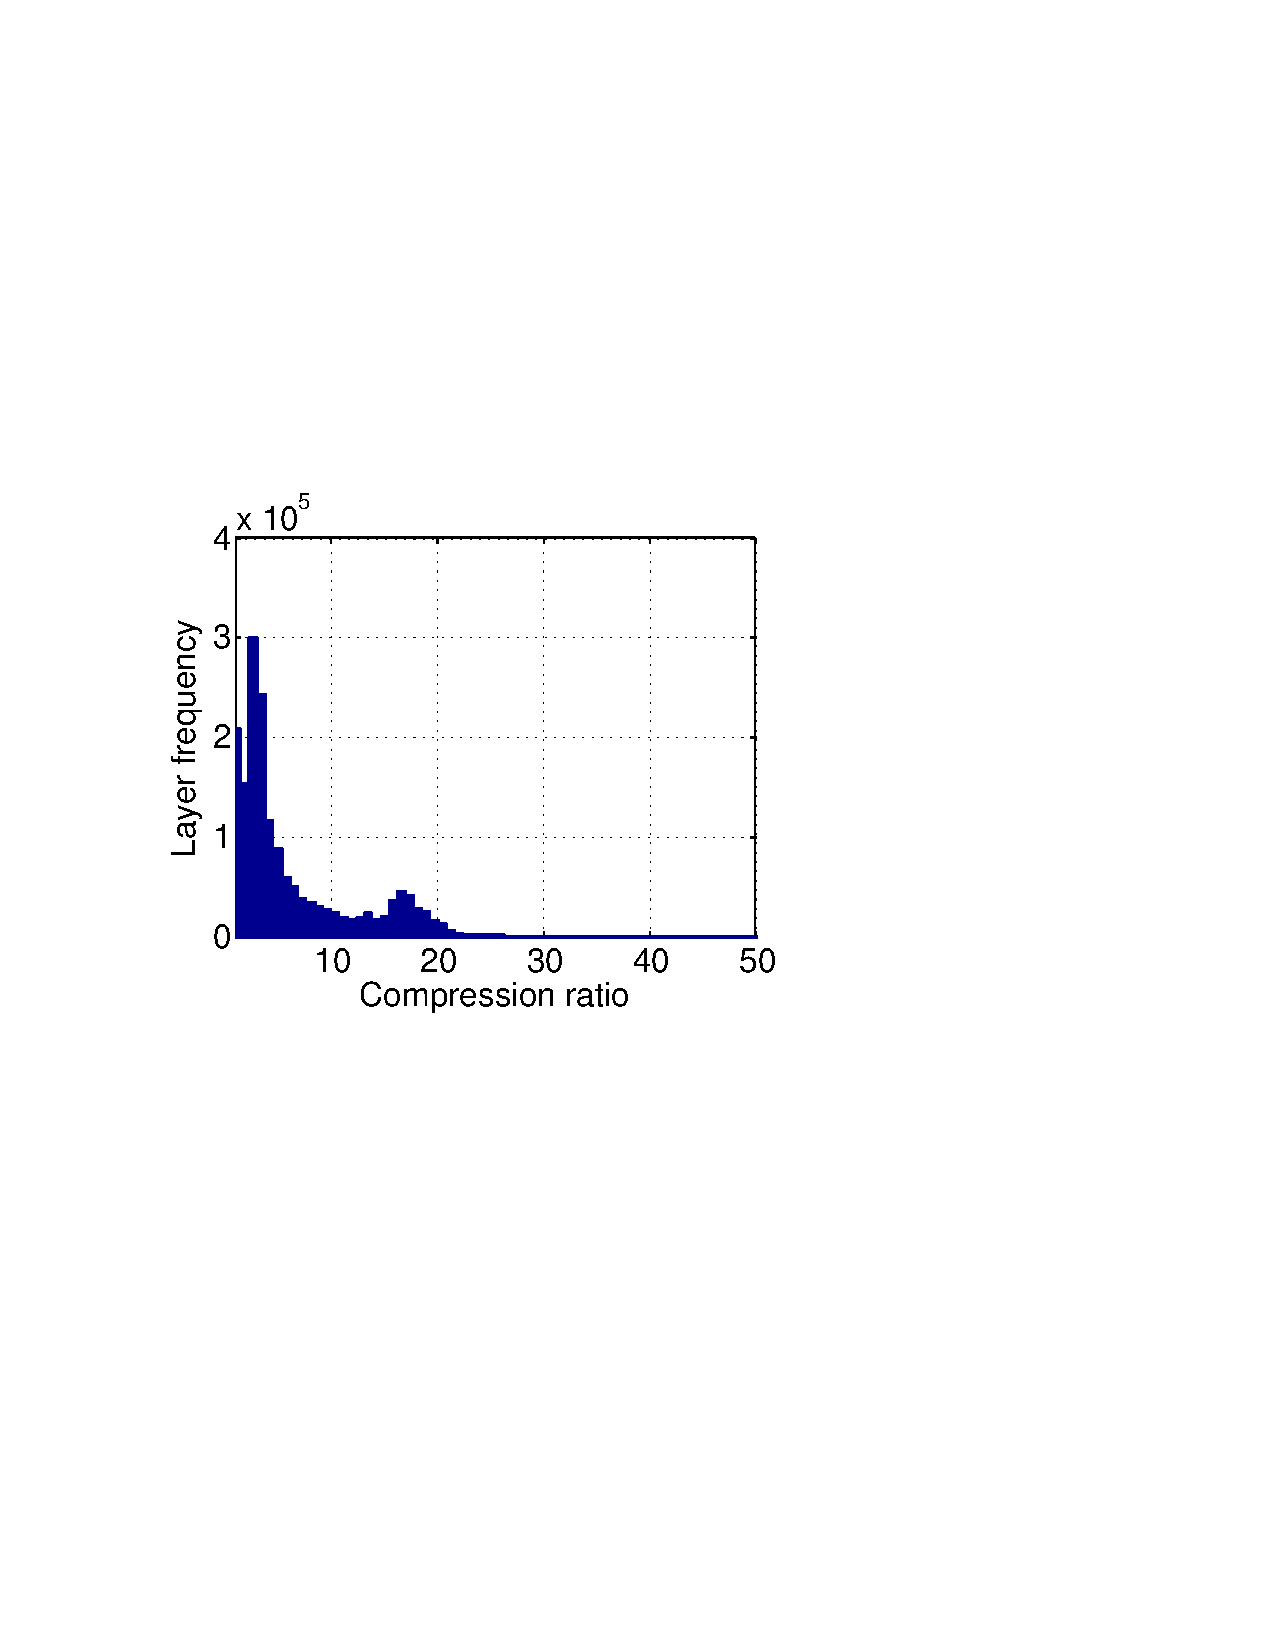
\includegraphics[width=0.22\textwidth]{graphs/layer-compress-ratio-pdf.pdf}
	}
	\caption{Histogram of image and layer compression ratio.}
	\label{fig:reference-cnt}
\end{figure}

Figure~\ref{fig:compress-ratio} shows the compression ratio of the container
images.  We find that 90\% of the images have an uncompressed size less than
1.3 GB and compressed size of 0.4~GB.
%while compressed images are less than 0.48 GB. 
In the median, this decreases to 94MB and 17 MB, respectively.  The largest
uncompressed image is 498 GB which is a Ubuntu-based image.  High compression
ratio shows the potential of compression while distributing the container
images.  \nancomment{there is redundancy and avg compression ratio}

However looking at Figure~\ref{fig_hist_image} and Figure~\ref{fig_hist_layer}
we find that there are layers for which the compression ratio is zero. Doing
compression and uncompression of such layers incur additional overhead at
docker engine side.  For such layers, we suggest not to do compression.
Docker engine can use a hybrid approach to perform compression by compressing
only those layers which yield better compression ratio. This way user does
not need to uncompress the layer which incurs no advantage and further
reduce the container startup time. 

\subsection{Layer count per image}
\nancomment{more layer more matedata? overhead for union fs}

\begin{figure}[!t]
	\centering
	\subfigure[CDF of layer count per image]{\label{fig_reference_cnt_cdf}
		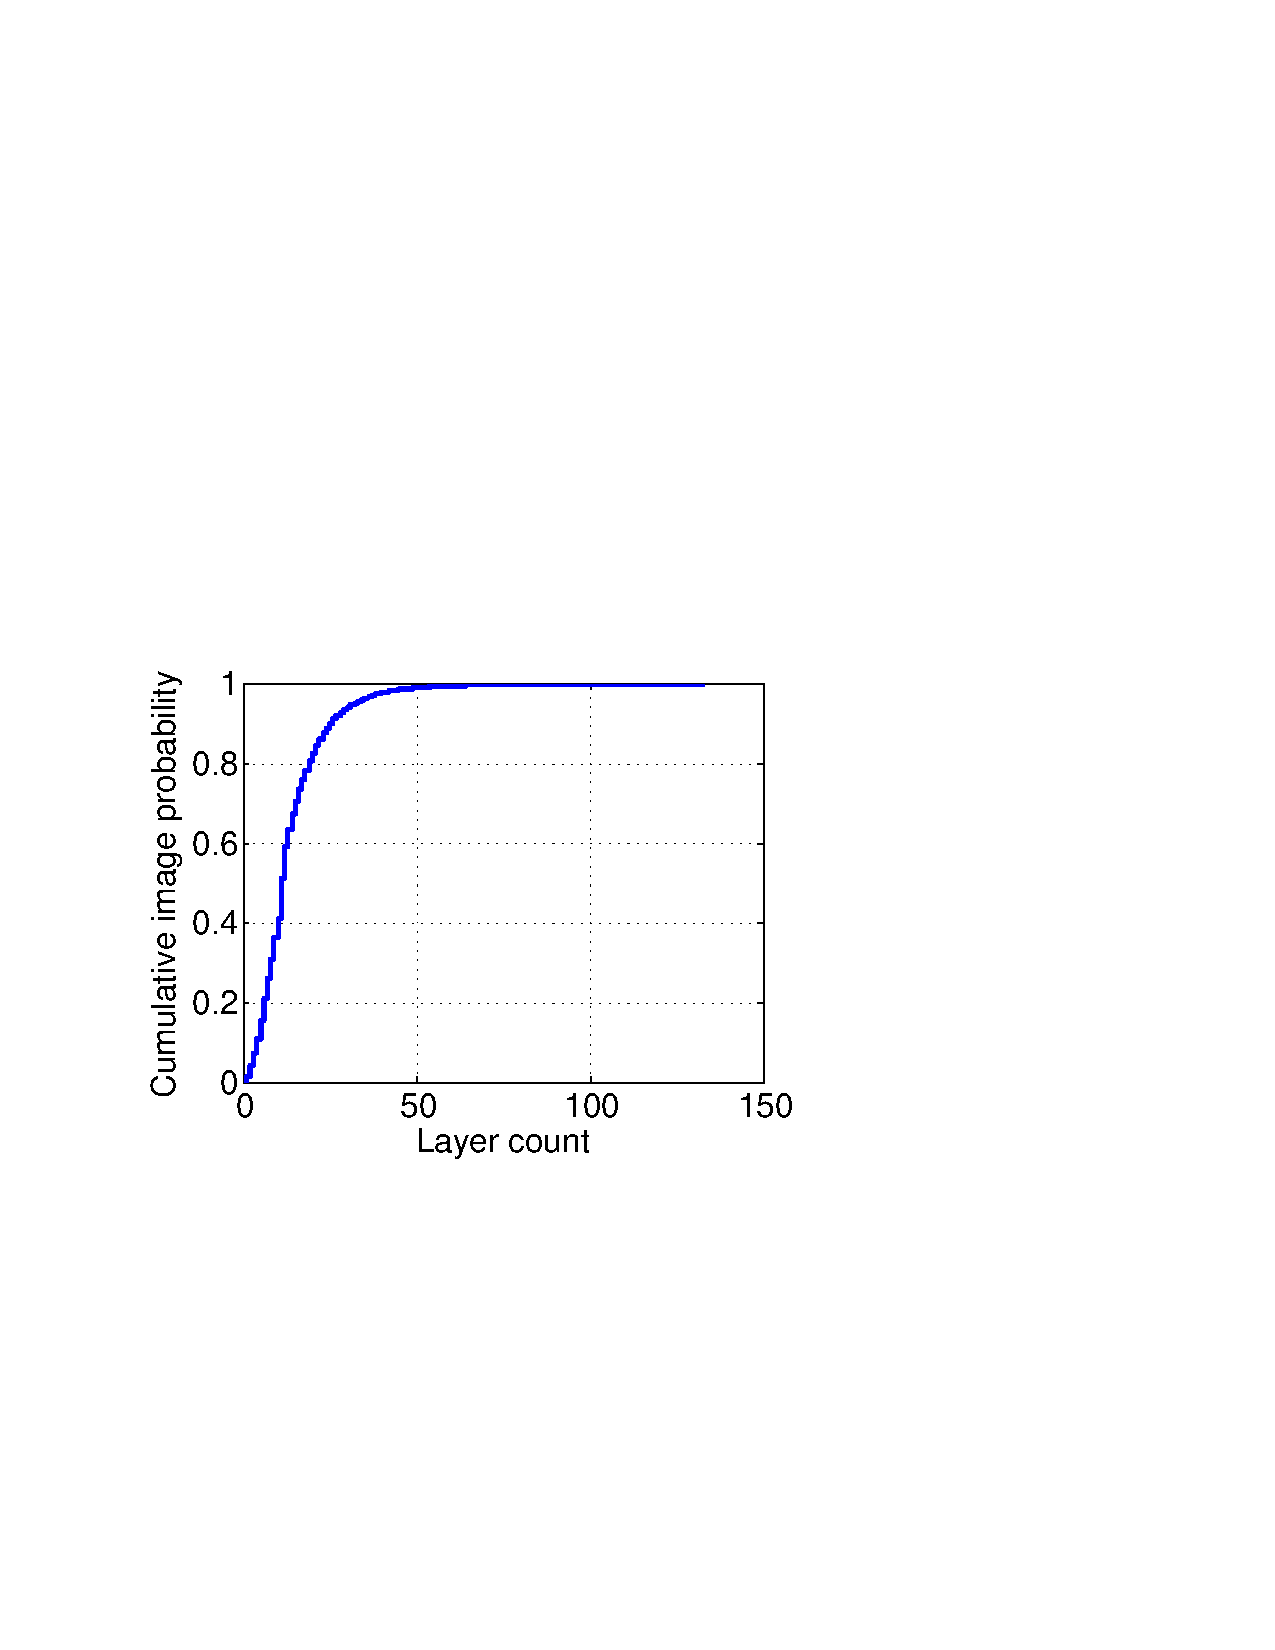
\includegraphics[width=0.215\textwidth]{graphs/image-layer-cnt}%
	}
	\subfigure[Histogram of layer count per image]{\label{fig_reference_cnt_pdf}
		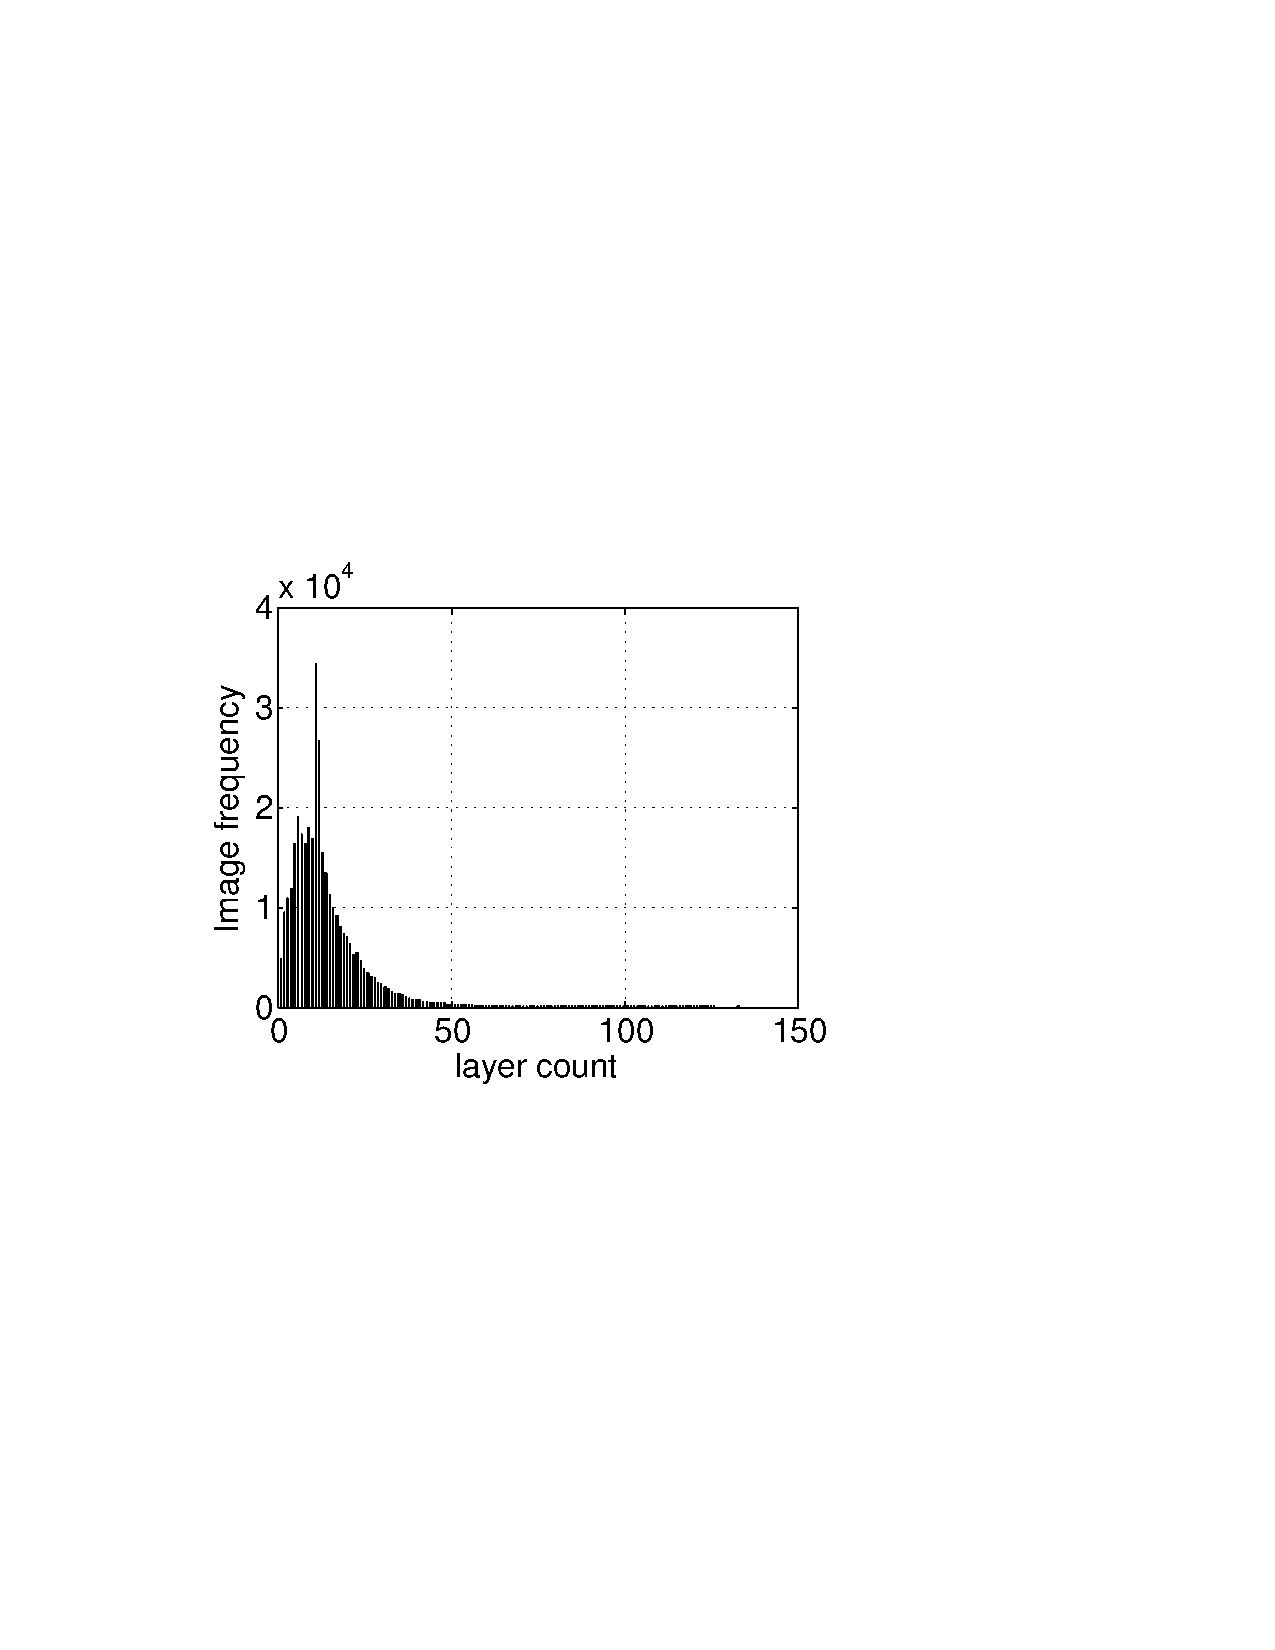
\includegraphics[width=0.21\textwidth]{graphs/image-layer-cnt-pdf.pdf}
	}
	\caption{Image size distribution}
	\label{fig:image-size}
\end{figure}

As discussed in~\ref{sec-image-layers}, images consist of a set of layers.
It is important to understand the layer count of the images as previous
work found that the number of layers can impact the performance of
I/O operations~\cite{slacker}. Therefore, we count the number of layers
per image and plot the CDF (see Figure~\ref{fig-layer-cnt})
and layer count frequencies (see Figure~\ref{fig_hist_layer_cnt})for all
Docker Hub images.

The results show that 90\% of the images have less than 18 layers while
half of the images have less than 8 layers. 8 layers is also the most
frequent layer value with 51,300 images consisting of exactly 8 layers.
The maximum layer count is 120 in the \textit{cfgarden/120-layer-image}.
We also find that there are 7,060 images which only consist of a single layer.

%\begin{figure}[!t]
	\centering
	\subfigure[CDF of layer reference count]{\label{fig_repeate_layer}
		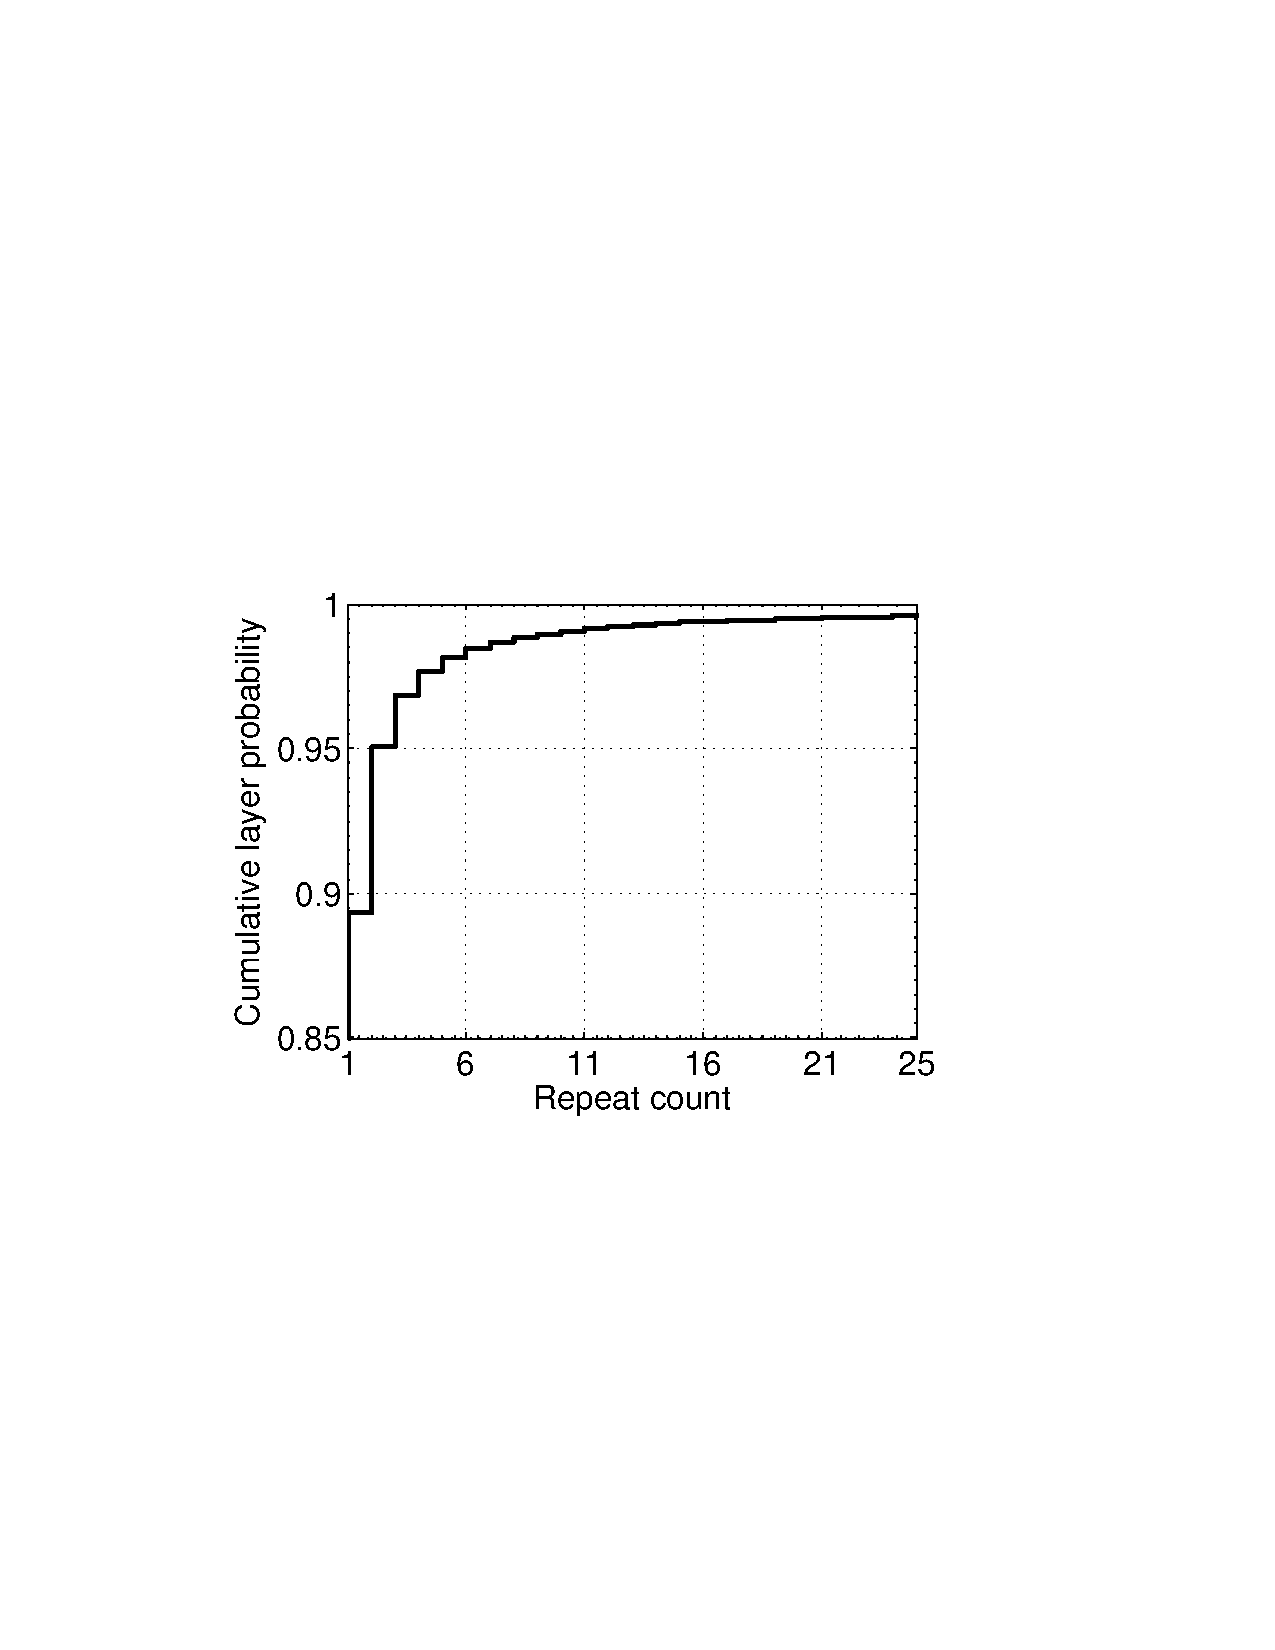
\includegraphics[width=0.23\textwidth]{graphs/repeate_layer.pdf}
	}
	\subfigure[Histogram of layer reference count]{\label{fig_hist_repeate_layer}
		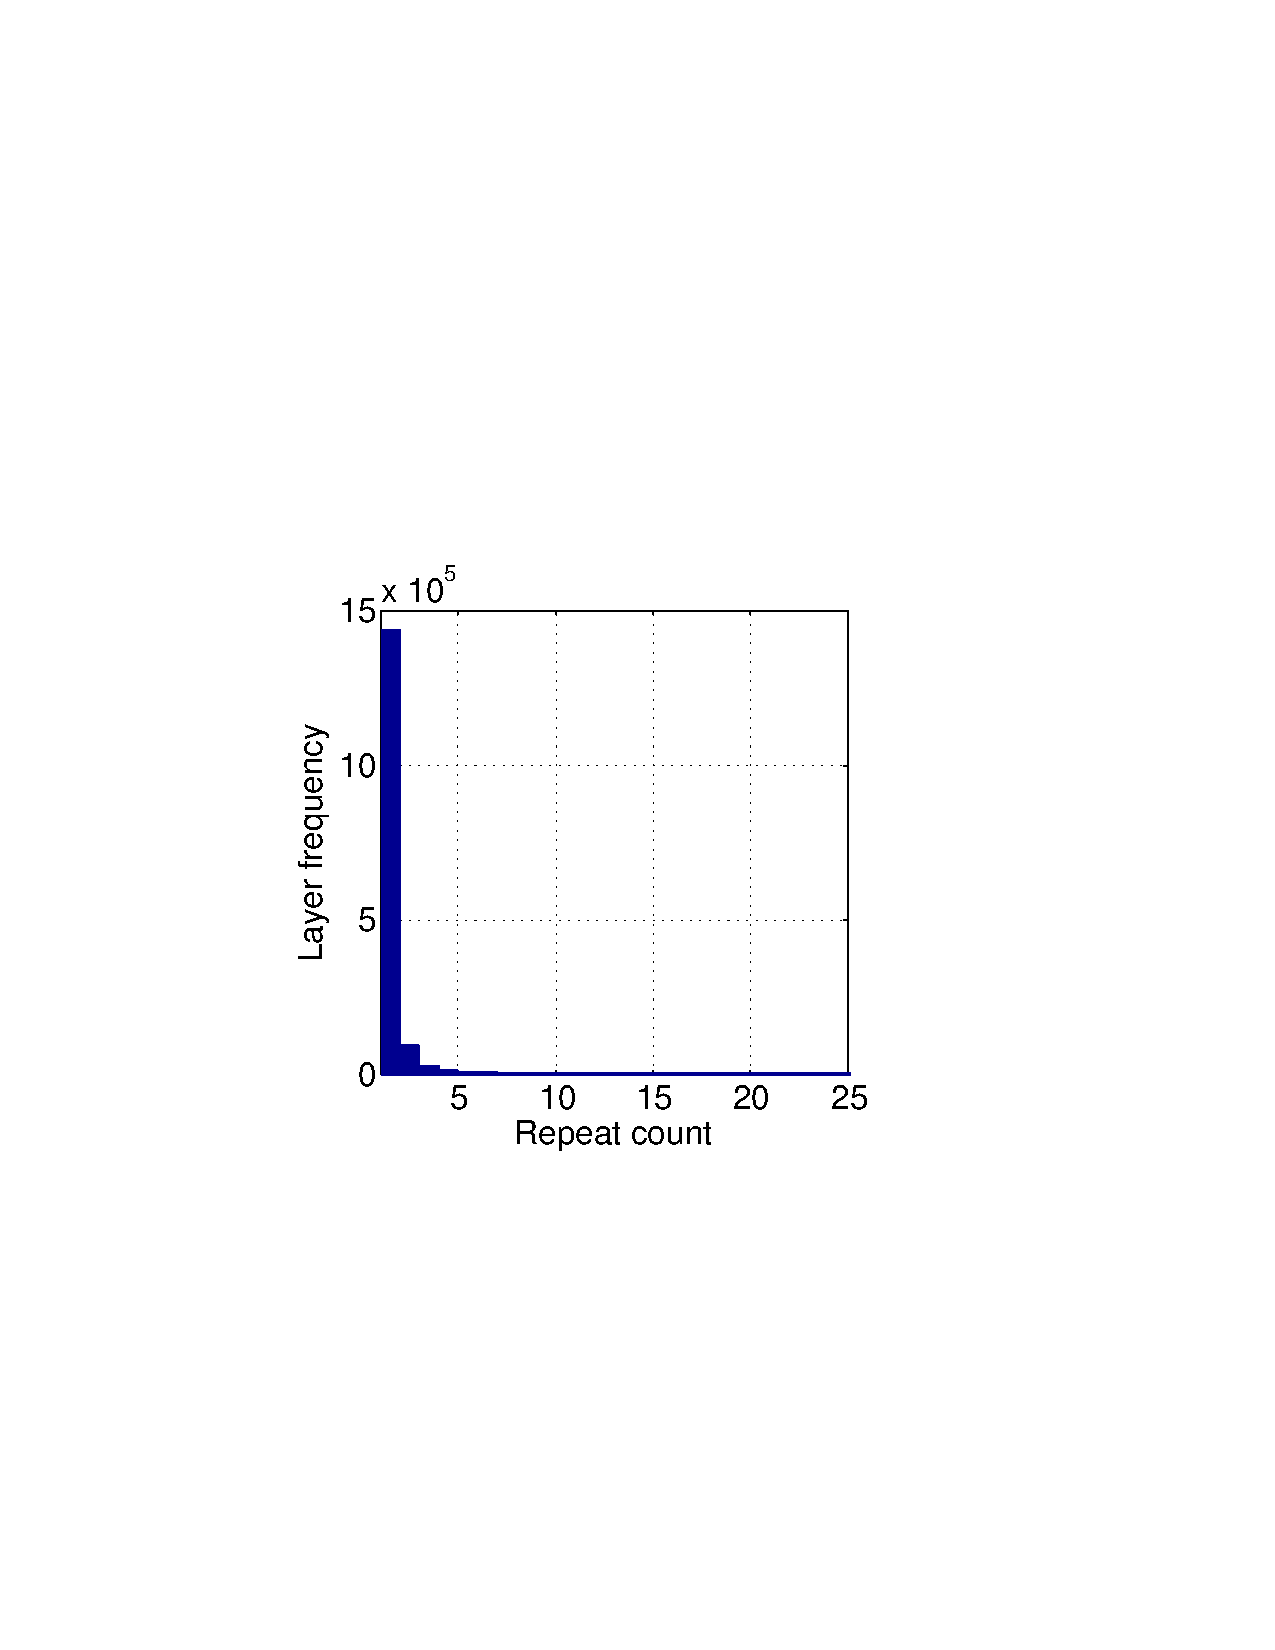
\includegraphics[width=0.223\textwidth]{graphs/hist_repeate_layer.pdf}
	}
	\caption{Layer reference counts across all images}
	\label{fig-repeat-layer-cnt}
\end{figure}

%\paragraph{Repeat layer count distribution}

An interesting question is what is the sharing rate of layers across images.
We analyze all image manifests and count for each layer, how many times it
is referenced by an image. Figure~\ref{fig_repeate_layer} shows that around 90\%
of layers are only reference by a single image while 95\% are reference by not
more than 2 images.
%99\% of layers are shared among less than 25 images. 
%
Figure~\ref{fig_hist_repeate_layer} shows the absolute values, revealing that
almost 1.5 million images are only referenced once. While there is again a large
spectrum of reference counts, the maximum is 33,428, the vast majority of layers
is not shared. This hints that the layer-based approach to improve storage
efficiency is barely utilized and there is room for improvement in how images

\subsection{Layer reference count}
\nancomment{should create more shared layers to remove duplicates}

\begin{figure}
	\centering
	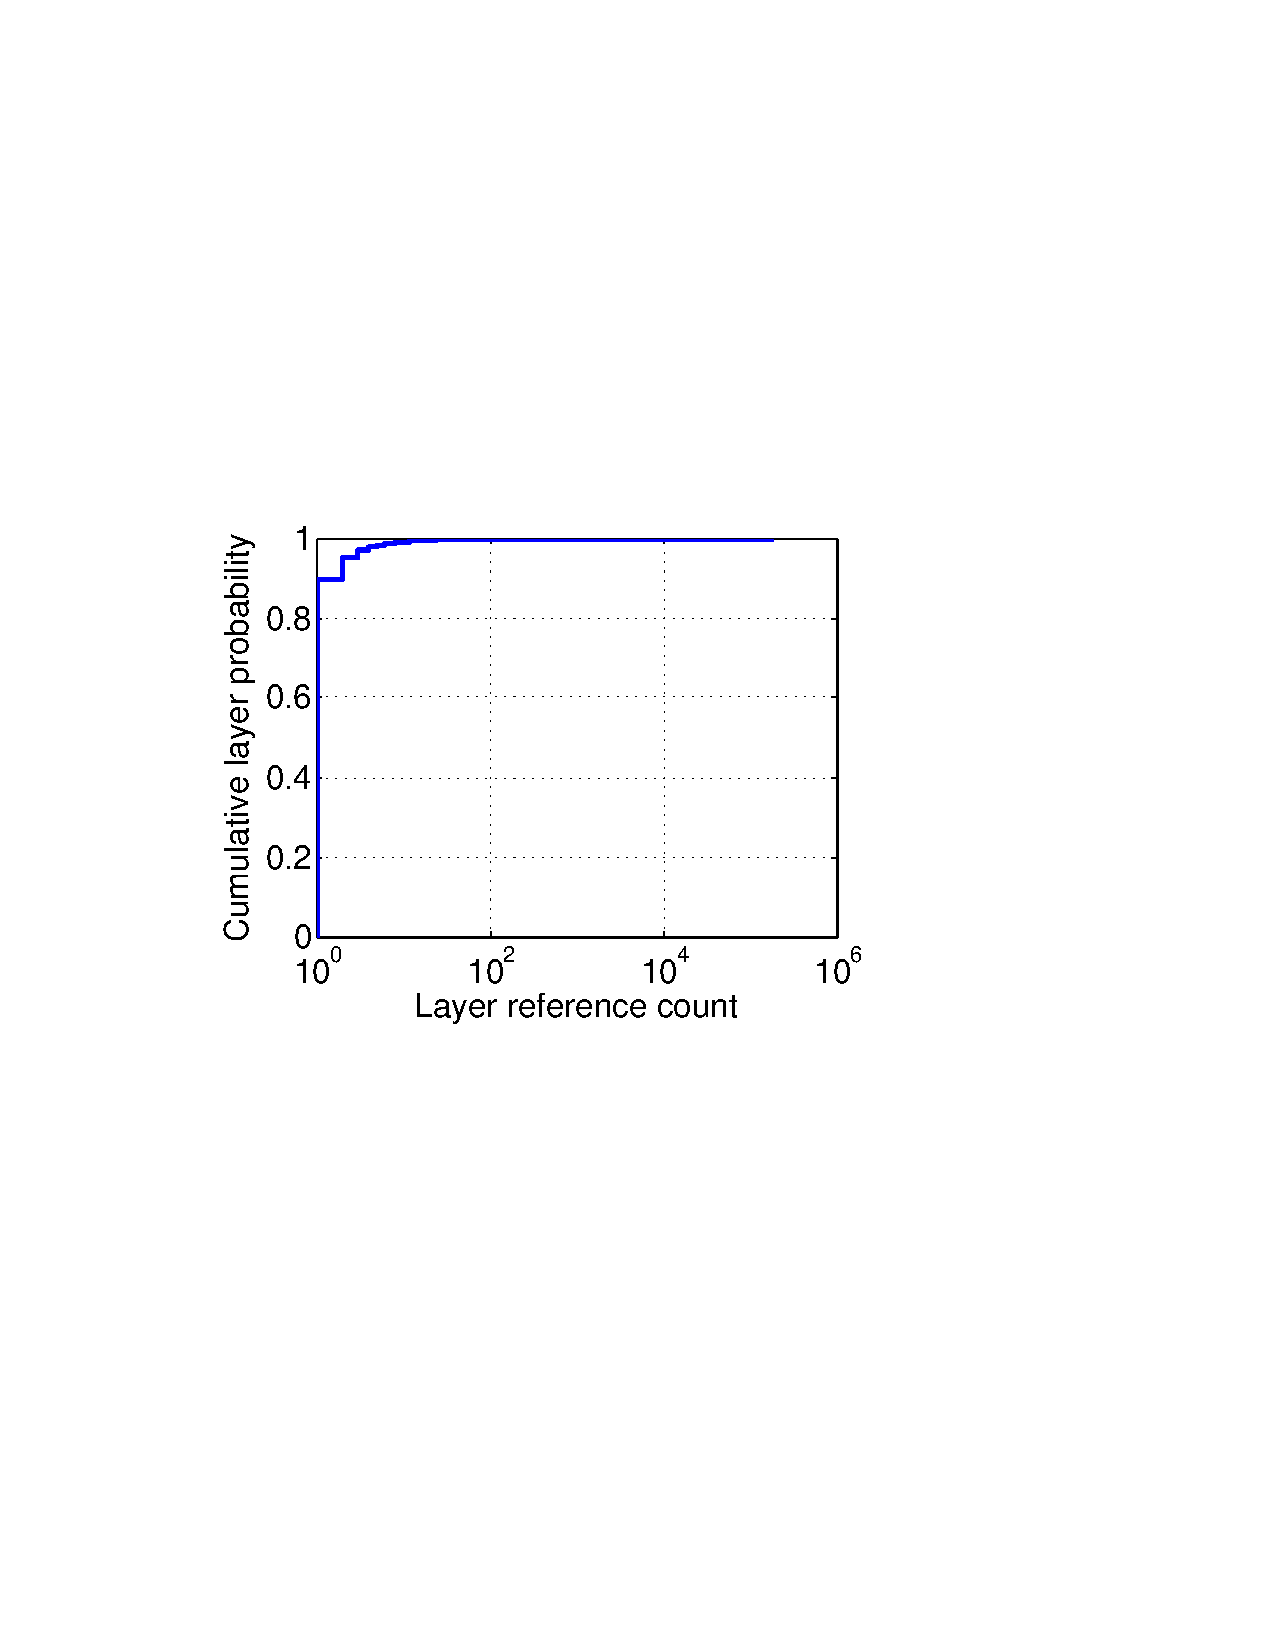
\includegraphics[width=0.21\textwidth]{graphs/shared-cnt-cdf.pdf}
	\caption{CDF of layer reference count.
	}
	\label{fig:reference-cnt}
\end{figure}

\subsection{Directory count}
\nancomment{how union fs handle so large dirs}
\begin{figure}
	\centering
	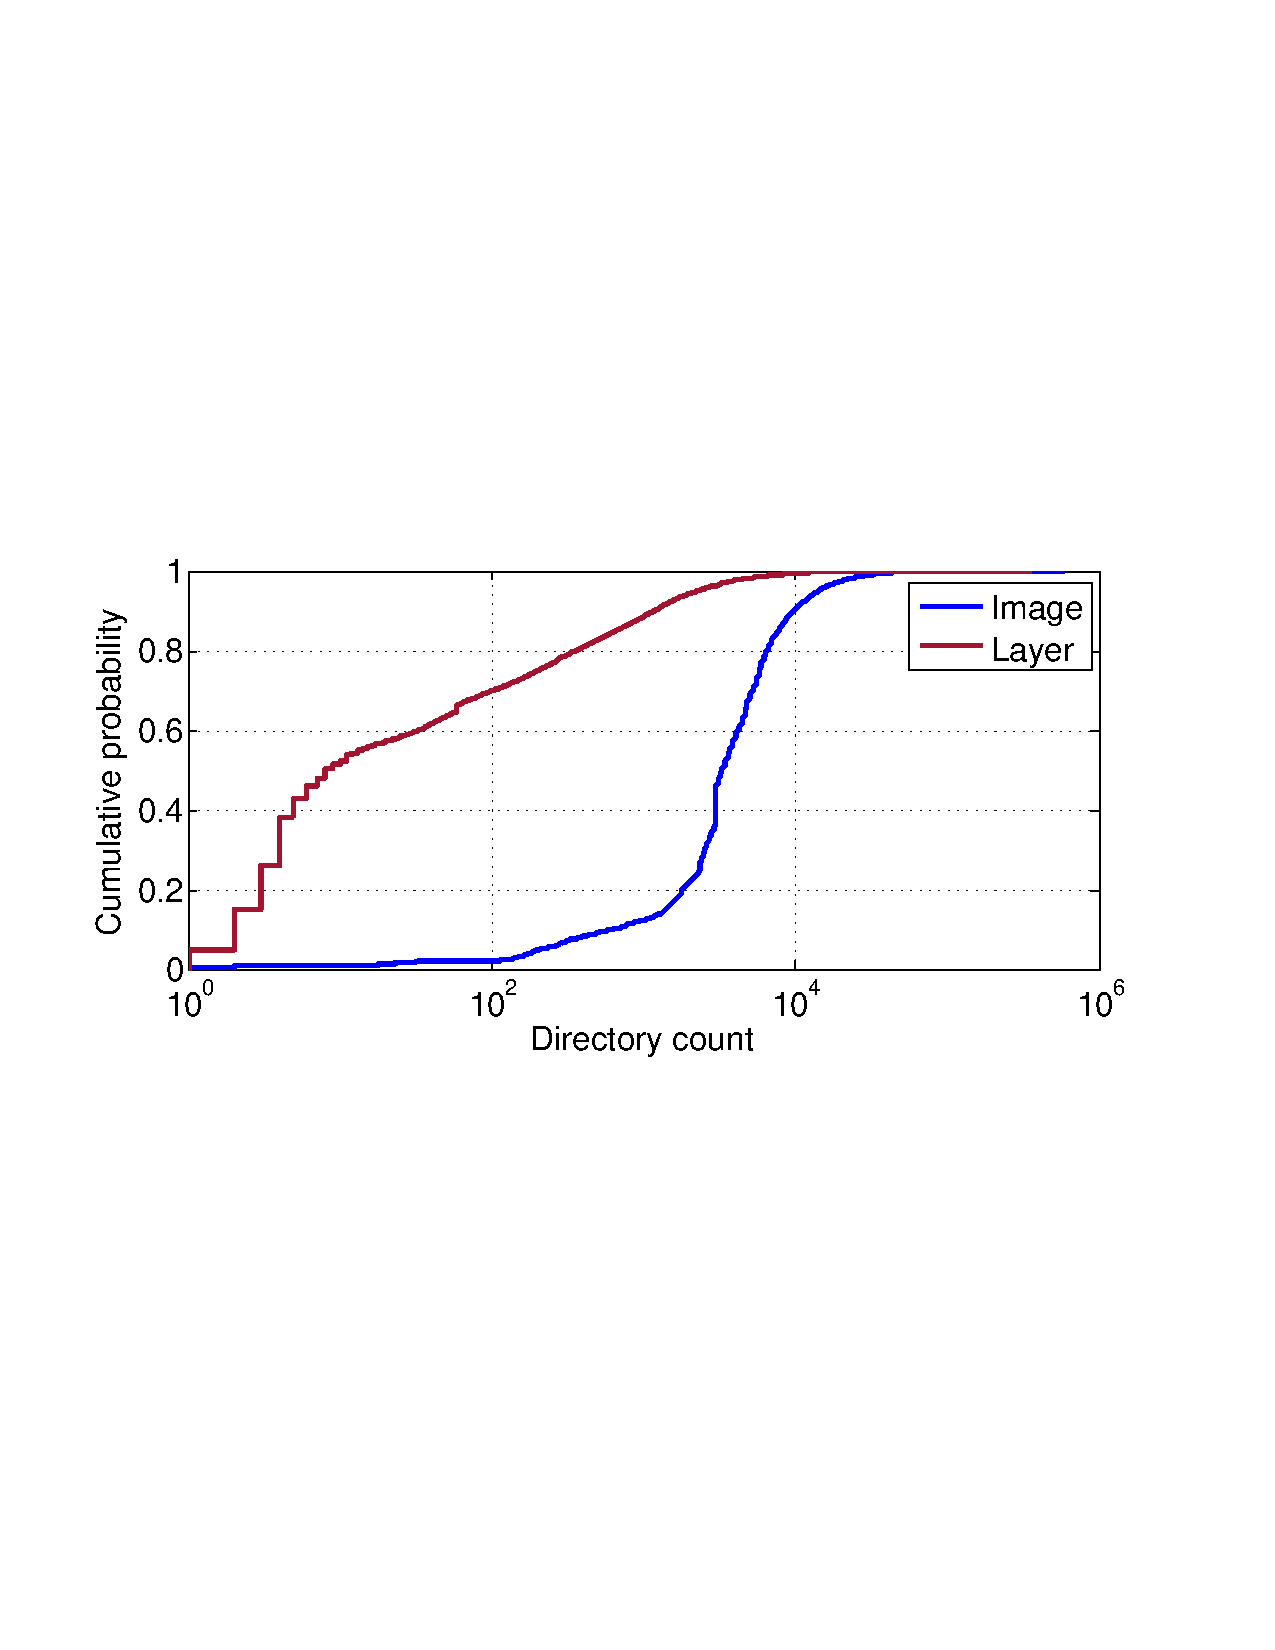
\includegraphics[width=0.4\textwidth]{graphs/dir-cnt-cdf.pdf}
	\caption{CDF of directory count per image/layer.
	}
	\label{fig:reference-cnt}
\end{figure}

\begin{figure}[!t]
	\centering
	\subfigure[Histogram of directory count per image]{\label{fig_reference_cnt_cdf}
		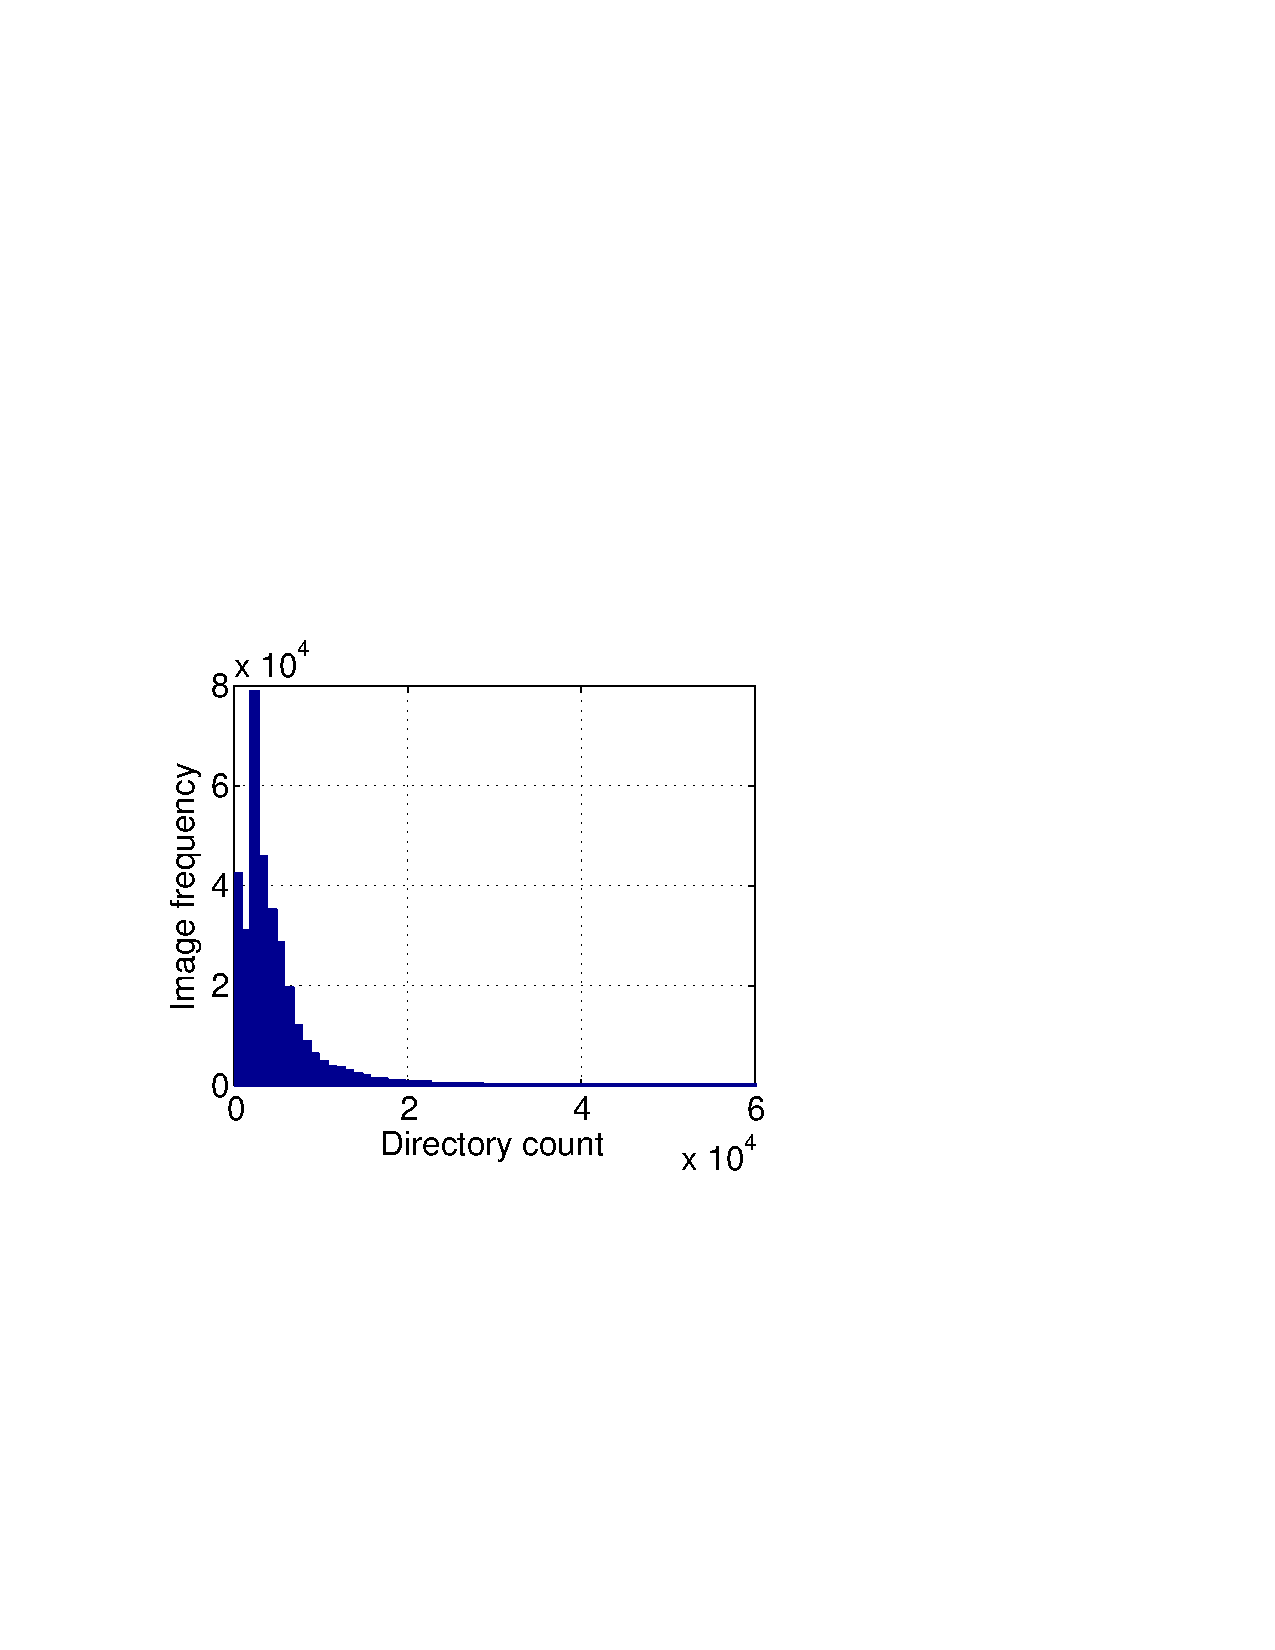
\includegraphics[width=0.2\textwidth]{graphs/image-dir-cnt-pdf.pdf}%
	}
	\subfigure[Histogram of directory count per layer]{\label{fig_reference_cnt_pdf}
		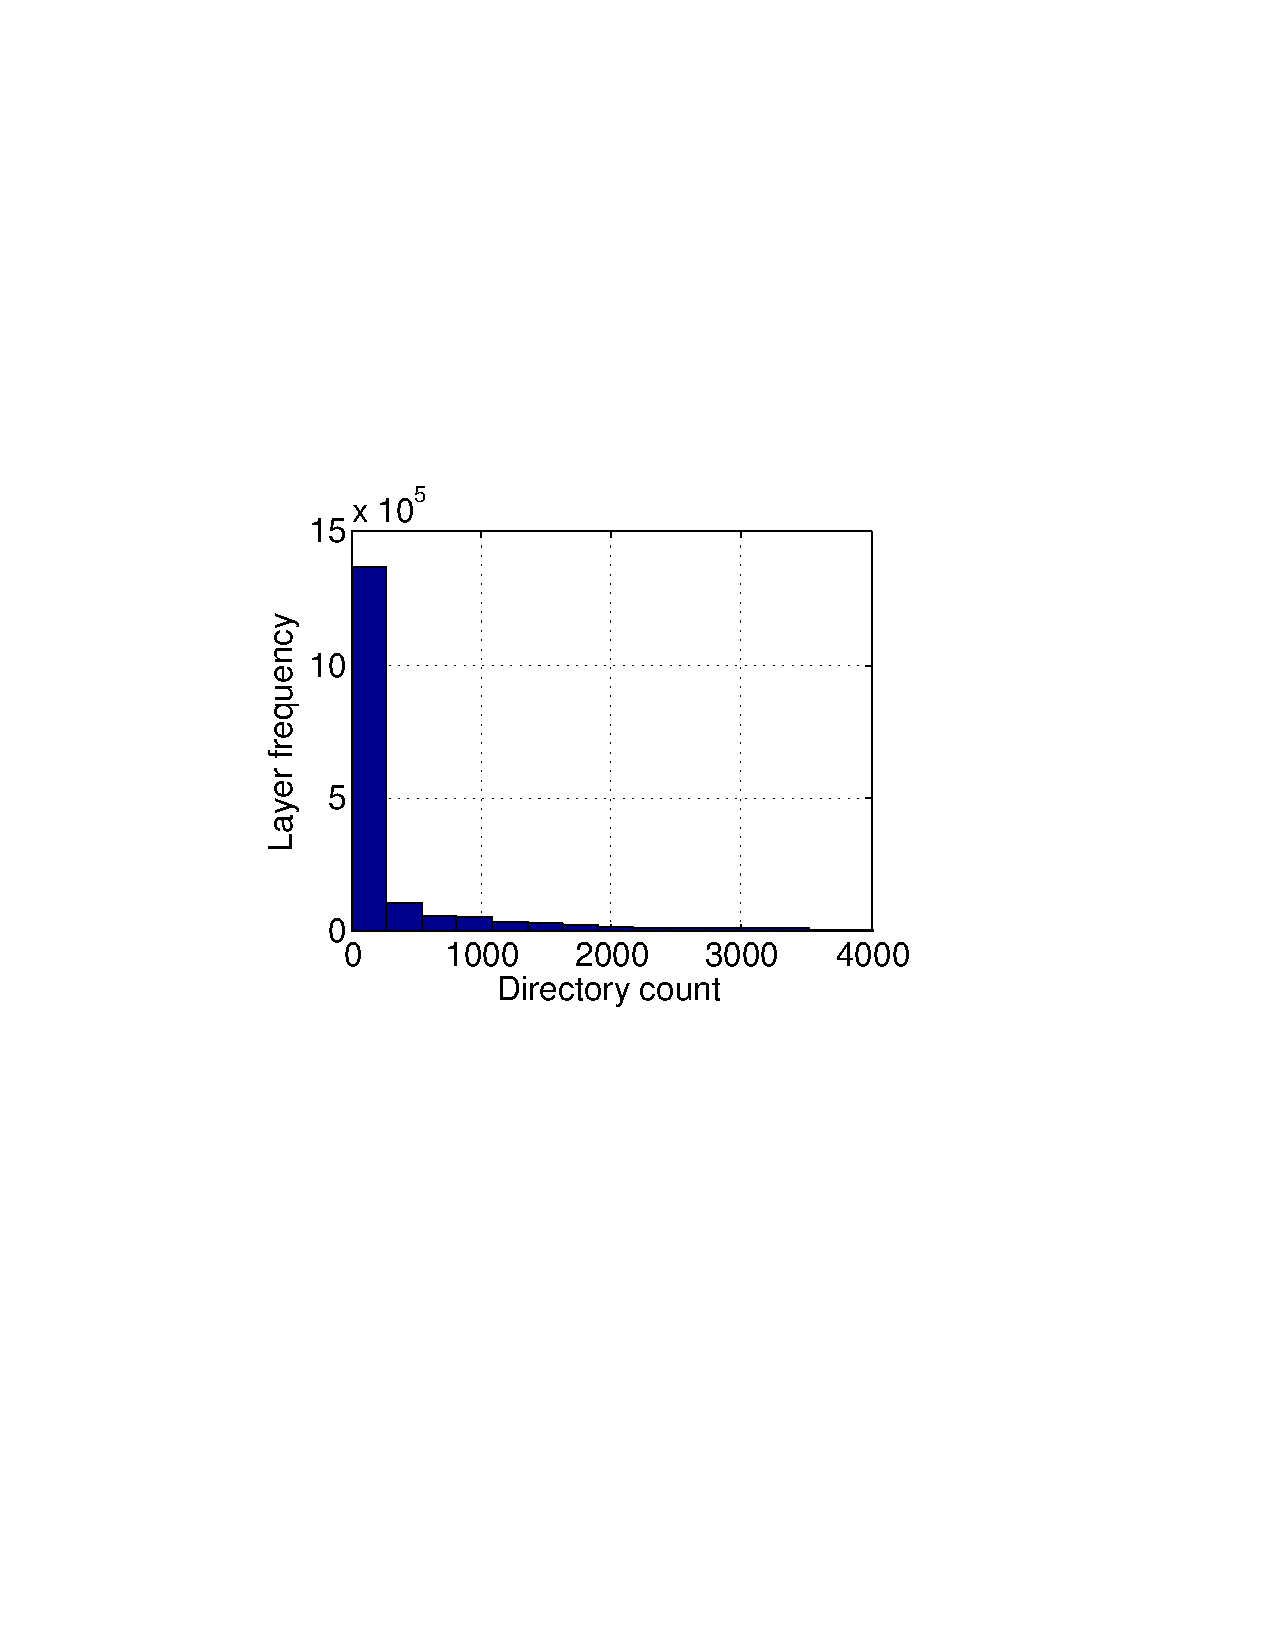
\includegraphics[width=0.22\textwidth]{graphs/layer-dir-cnt.pdf}
	}
	\caption{Histogram of directory count distribution}
	\label{fig:reference-cnt}
\end{figure}

Lastly, we look at the directory (see Figure~\ref{fig-dir}) and file counts
(see Figure~\ref{fig-file}) in images to determine if deploying
images requires handling of large amounts of metadata. Looking at directories,
we see that 90\% of images have less than 7,344 directories while the median
is at 296. For files, 90\% of images have less than 64,780 files with a median
of 1,090.

This is consistent with our analysis of layer-based file and directory counts
and the number of layers per image. Again, we conclude that most images
do not require an extensive amount of metadata when being deployed as file and
directory counts are low except for few outliers.

We characterize layer sizes using two different different metrics:
%
1)~Compressed Layer Size (CLS)---the format a layer is stored in the registry or
transferred to a client;
%
%2)~Archived Layer Size (ALS)---layer in decompressed but archived format;
%
and 2)~Files in Layer Size (FLS)---the sum of the sizes of the uncompressed files contained
in the layer.
%
Figure~\ref{fig_layer_size_cdf} shows the CDF of the two metrics.


%The ALS and FLS curves are, expectedly, close to each other (within 5\% for
%any given layer size) while compressed layers are typically smaller.
%j
We see that 90\% of the layers are smaller than 177~MB in uncompressed 
format and smaller than 63~MB in compressed format.
%
Interestingly, about half of the layers are smaller than 4~MB, independent
of the format. That means that the registry stores a large number of
small layers which cannot benefit from compression.

To analyze the frequencies, we zoom into the 0--128~MB range
(see Figure~\ref{fig_hist_layer_size}).
%
More than 1 million and 800,000 layers are smaller than 5~MB
in compressed and uncompressed format, respectively. Beyond that,
the frequency drops rapidly and we only see around 100,000 layers
between 5~MB and 15~MB.

%\begin{figure}[!t]
	\centering
	\subfigure[CDF of compression ratio]{\label{fig_cdf_compression_ratio}
		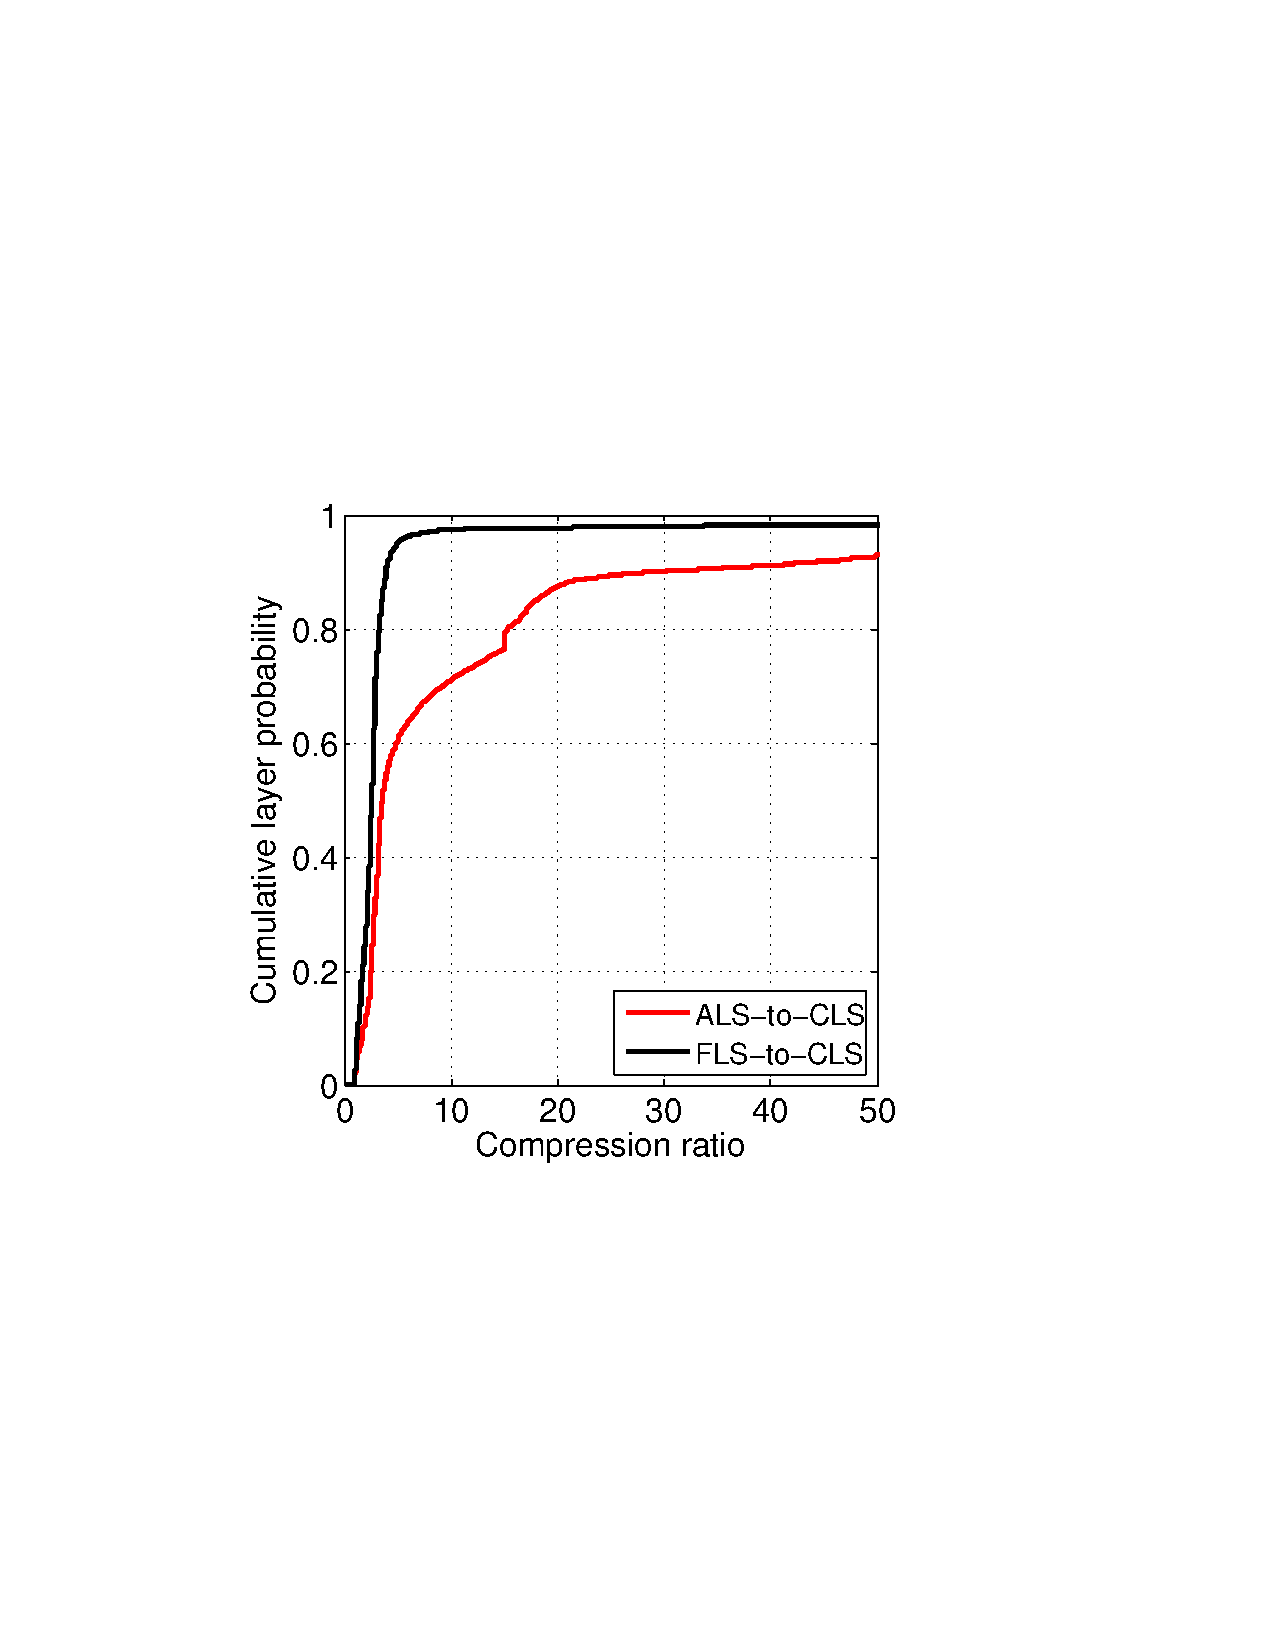
\includegraphics[width=0.23\textwidth]{graphs/cdf_compression_ratio.pdf}
	}
	\subfigure[Histogram of comp. ratios]{\label{fig_his_compression_ratio}
		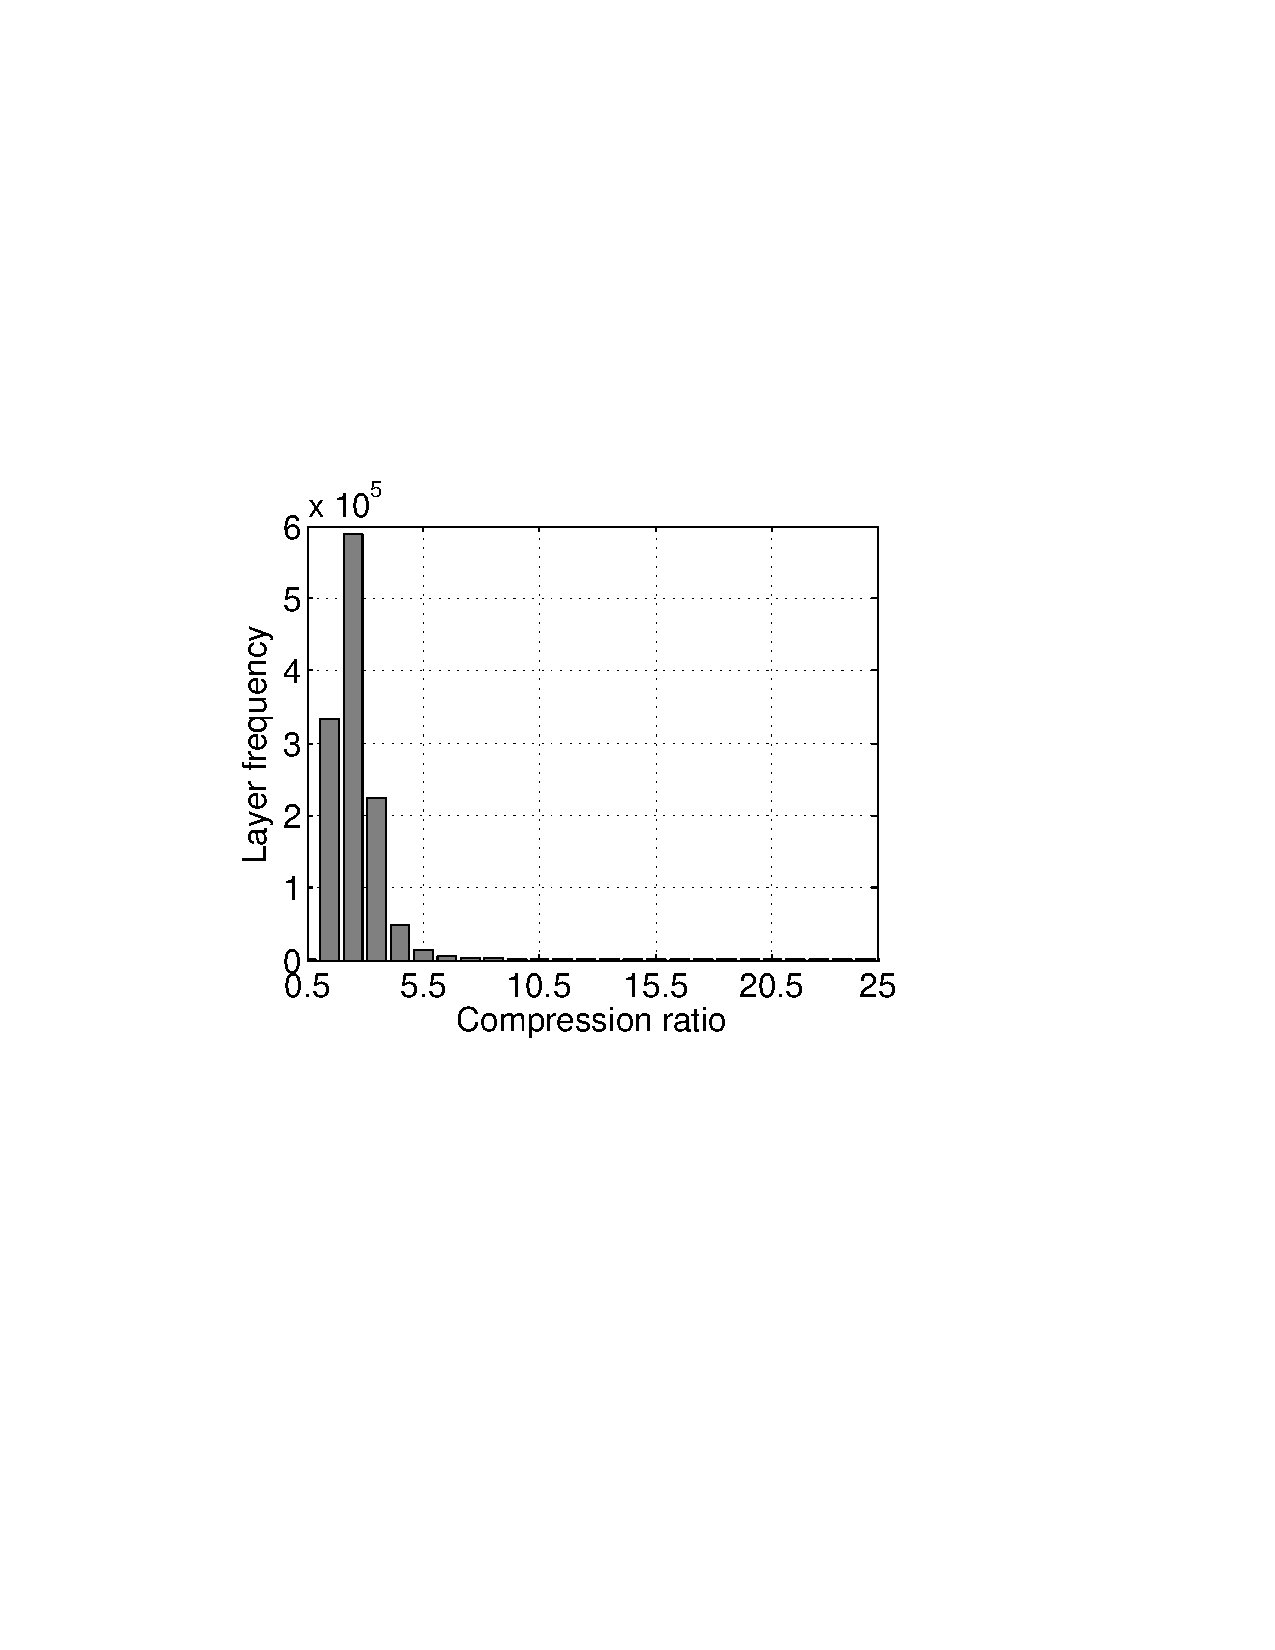
\includegraphics[width=0.223\textwidth]{graphs/his_compression_ratio.pdf}
	}
	\caption{Layer compression ratio distribution
	%\vcomment{Different colors are used in figure (a) and (b) FLS/CLS\nancomment{will address later}}
	}
	\label{fig-compression-ratio}
\end{figure}


%\paragraph{Layer compression ratios}

To further study the sizes and the impact of compression, we calculate
the FLS-to-CLS compression ratios (see Figure~\ref{fig_cdf_compression_ratio}).
%
%The ALS-to-CLS ratio is generally greater than the FLS-to-CLS ratio
%because small files in layers get larger when combined in a tar archive.
%
90\% of layers have a  FLS-to-CLS ratio less than 4 and the median
compression ratio is 2.6. The largest compression ratio is 1026.
%
%Half of the layers have a compression ratio (both ALS-to-CLS and
%FLS-to-CLS) around 3.
%
%
%The maximum FLS-to-CLS is 512,930 and maximum ALS-to-CLS is 1026.
%
Looking at the histogram (see Figure~\ref{fig_his_compression_ratio}), we see
that around 600,000 layers have a compression ratio of between 2 and 3 while more than
300,000 between 1 and 2.
%
%Two peaks in the graph correspond to 587,000 layers that have the FLS-to-CLS ratio of 3
%and 331,000 layers that have the ALS-to-CLS ratio of 3.

Our size analysis reveals an interesting trade-off. Compression is computationally
expensive and is one of the major sources of latency when pulling an image from Docker Hub~\cite{slacker}.
As the majority of layers is small and has low compression ratios, it can
be beneficial to store small layers uncompressed in the registry to reduce pull latencies.

\paragraph{Layer depth}
\nancomment{fs metadata overhead}

\begin{figure}[!t]
	\centering
	\subfigure[CDF of layer depth]{\label{fig_reference_cnt_cdf}
		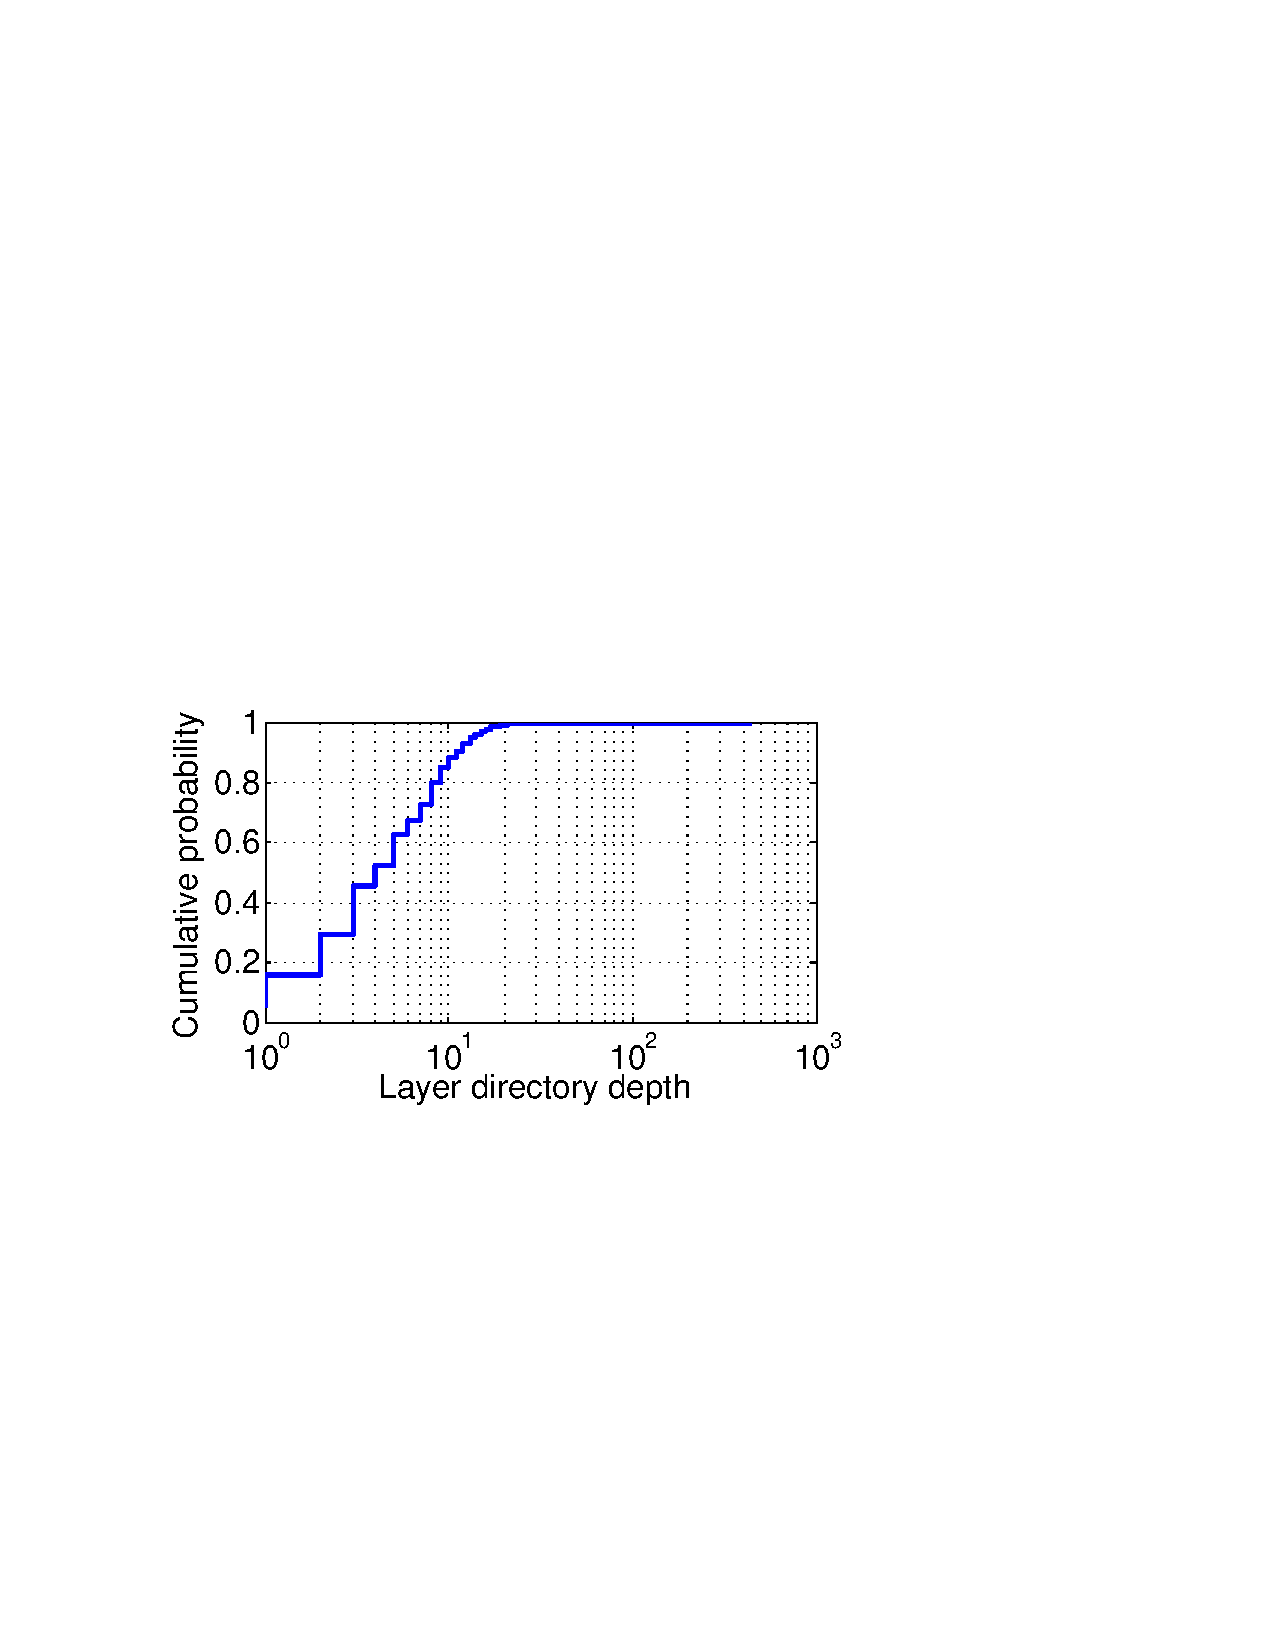
\includegraphics[width=0.21\textwidth]{graphs/layer-depth-cdf.pdf}%
	}
	\subfigure[Histogram of layer depth]{\label{fig_reference_cnt_pdf}
		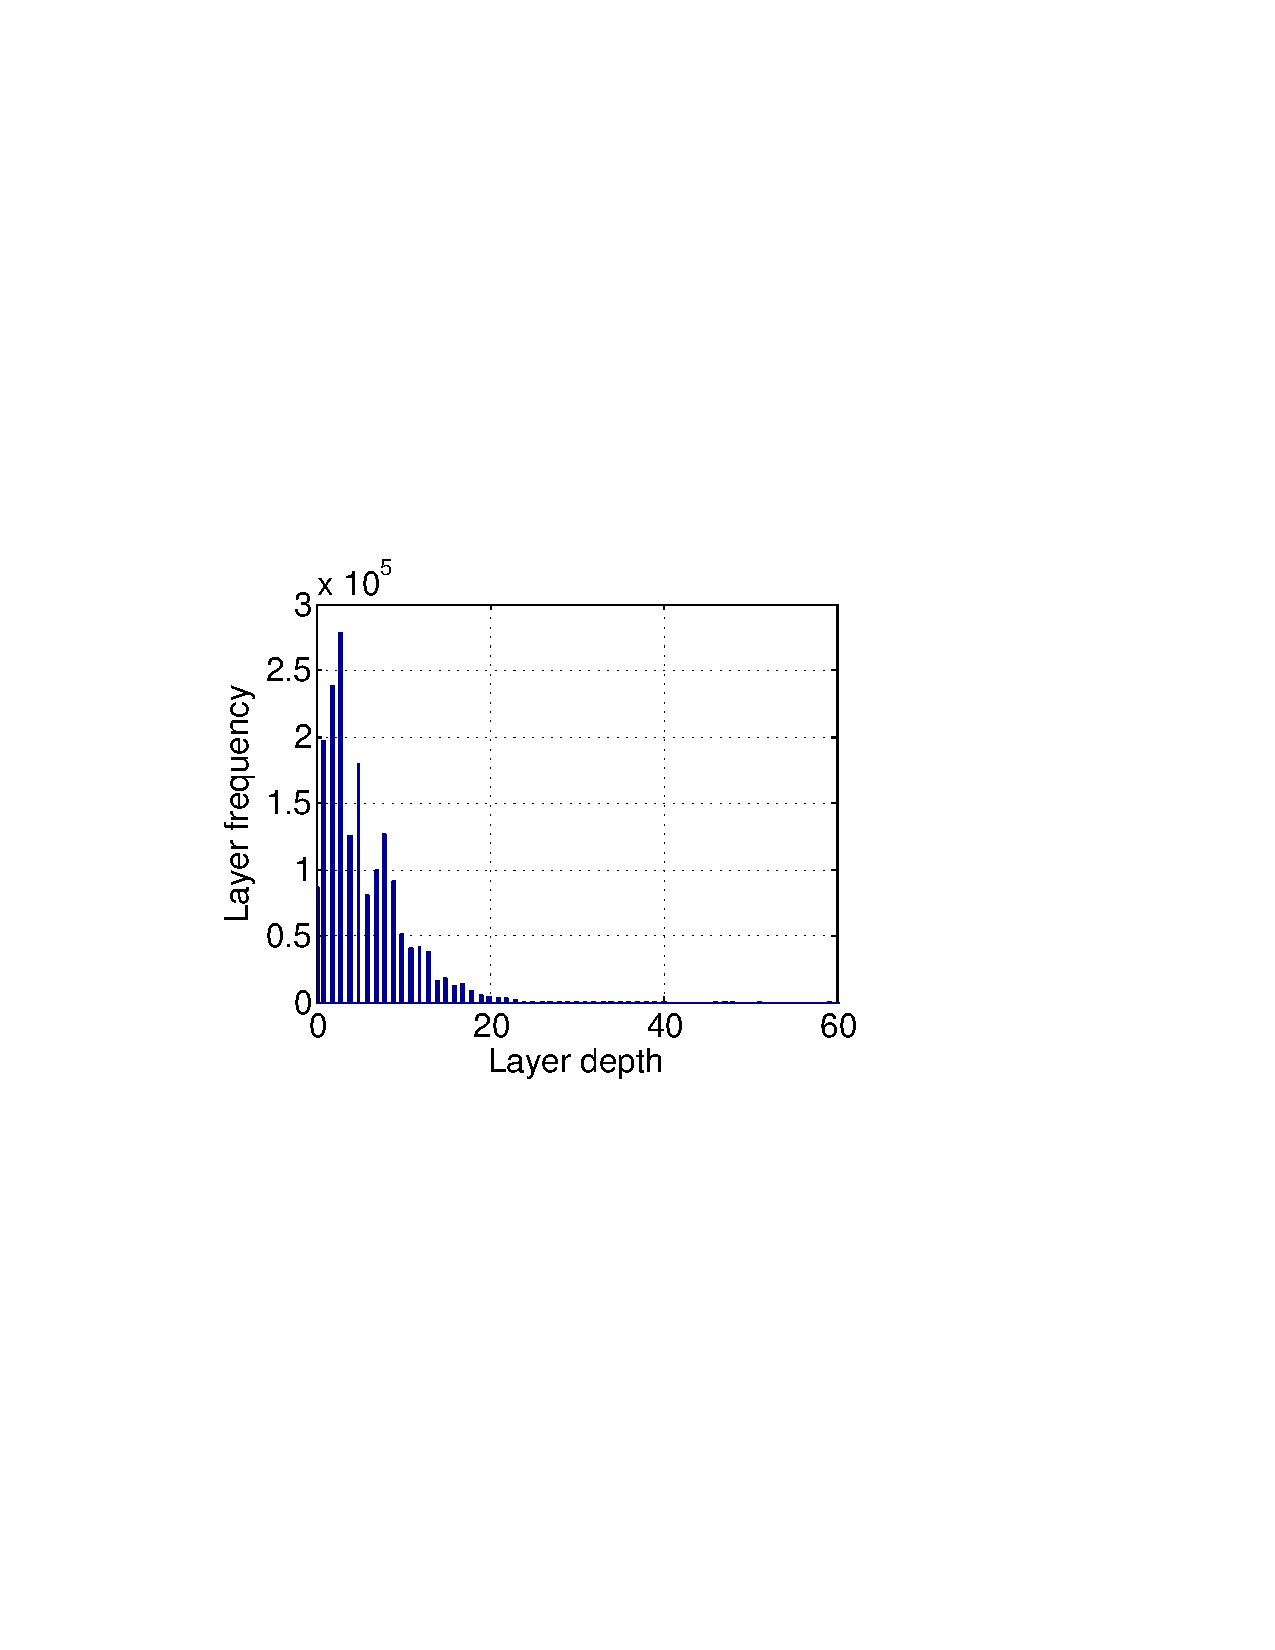
\includegraphics[width=0.21\textwidth]{graphs/layer-depth-pdf.pdf}
	}
	\caption{Layer depth distribution}
	\label{fig:reference-cnt}
\end{figure}

\subsection{File count} 
\nancomment{still metadata overhead}
\begin{figure}
	\centering
	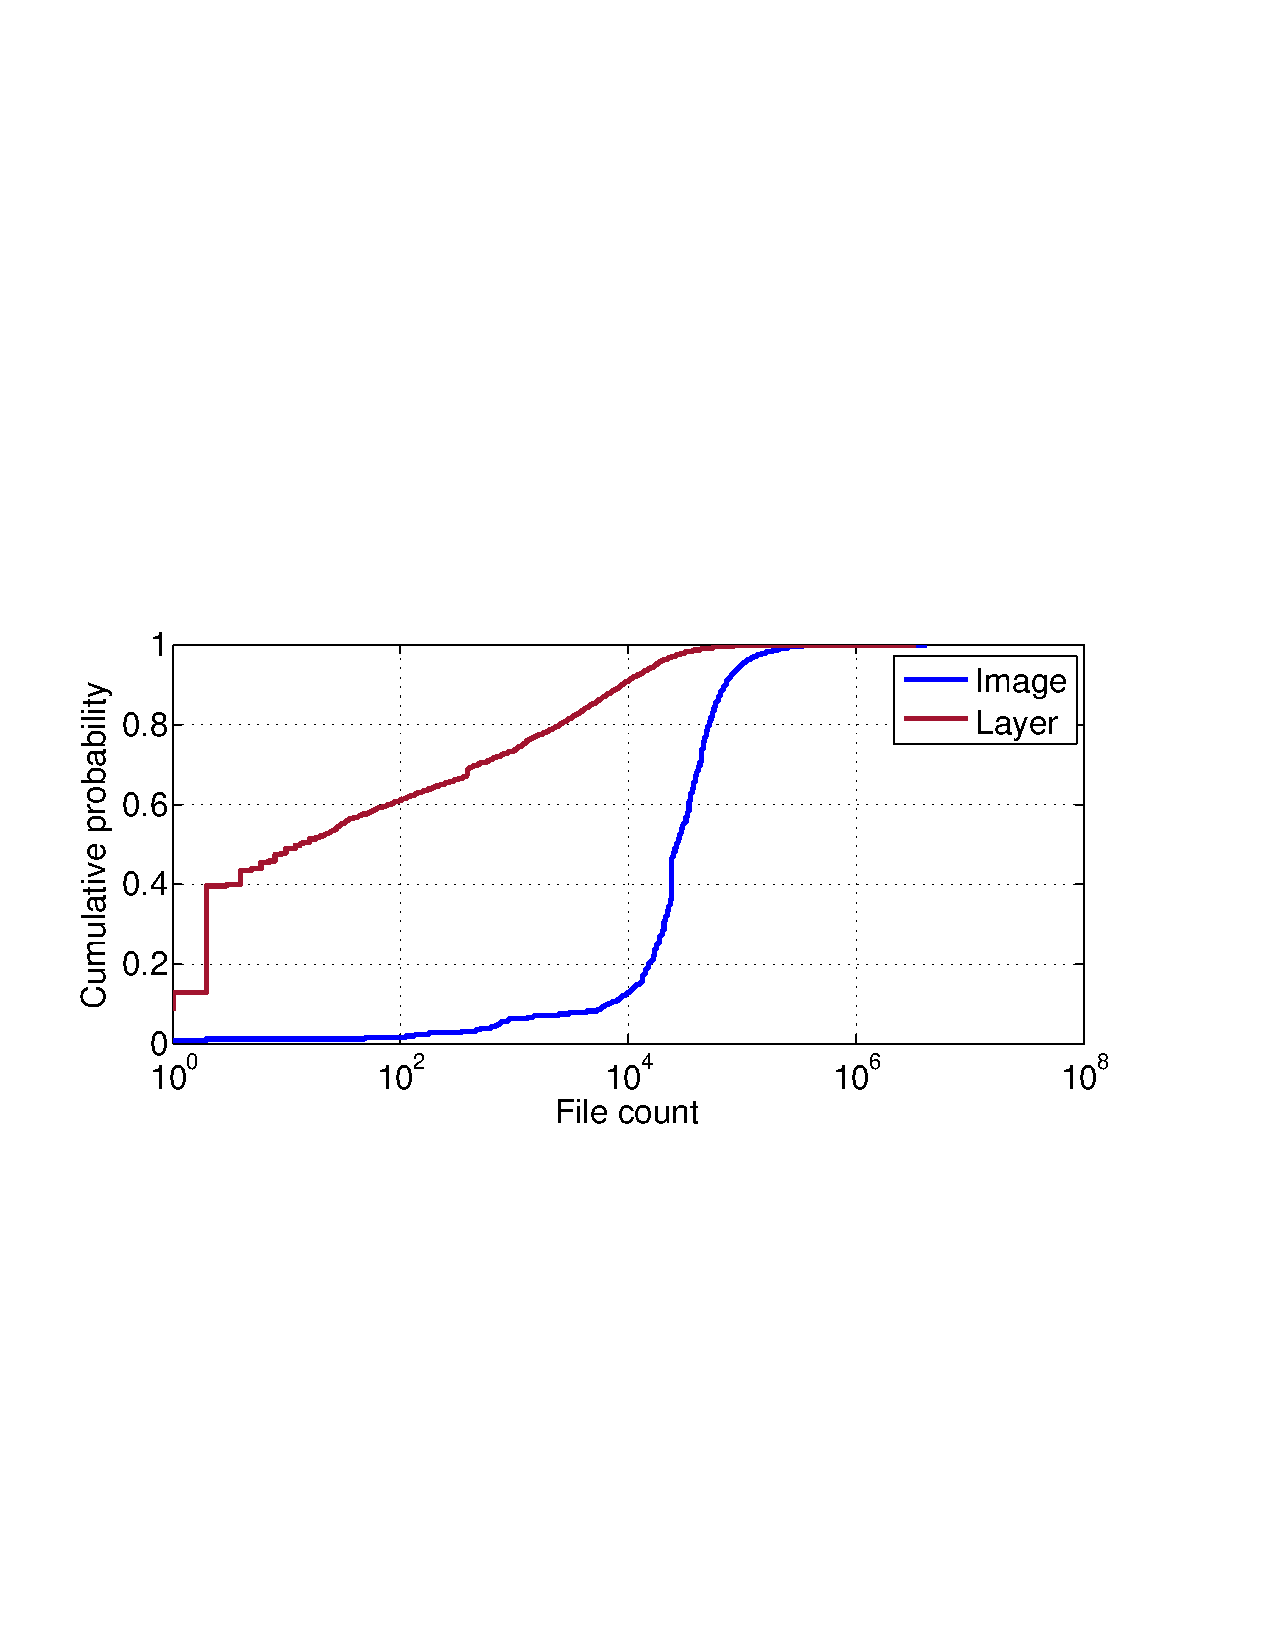
\includegraphics[width=0.4\textwidth]{graphs/file-cnt-cdf.pdf}
	\caption{CDF of file count per image/layer.
	}
	\label{fig:reference-cnt}
\end{figure}

\begin{figure}[!t]
	\centering
	\subfigure[Histogram of directory count per image]{\label{fig_reference_cnt_cdf}
		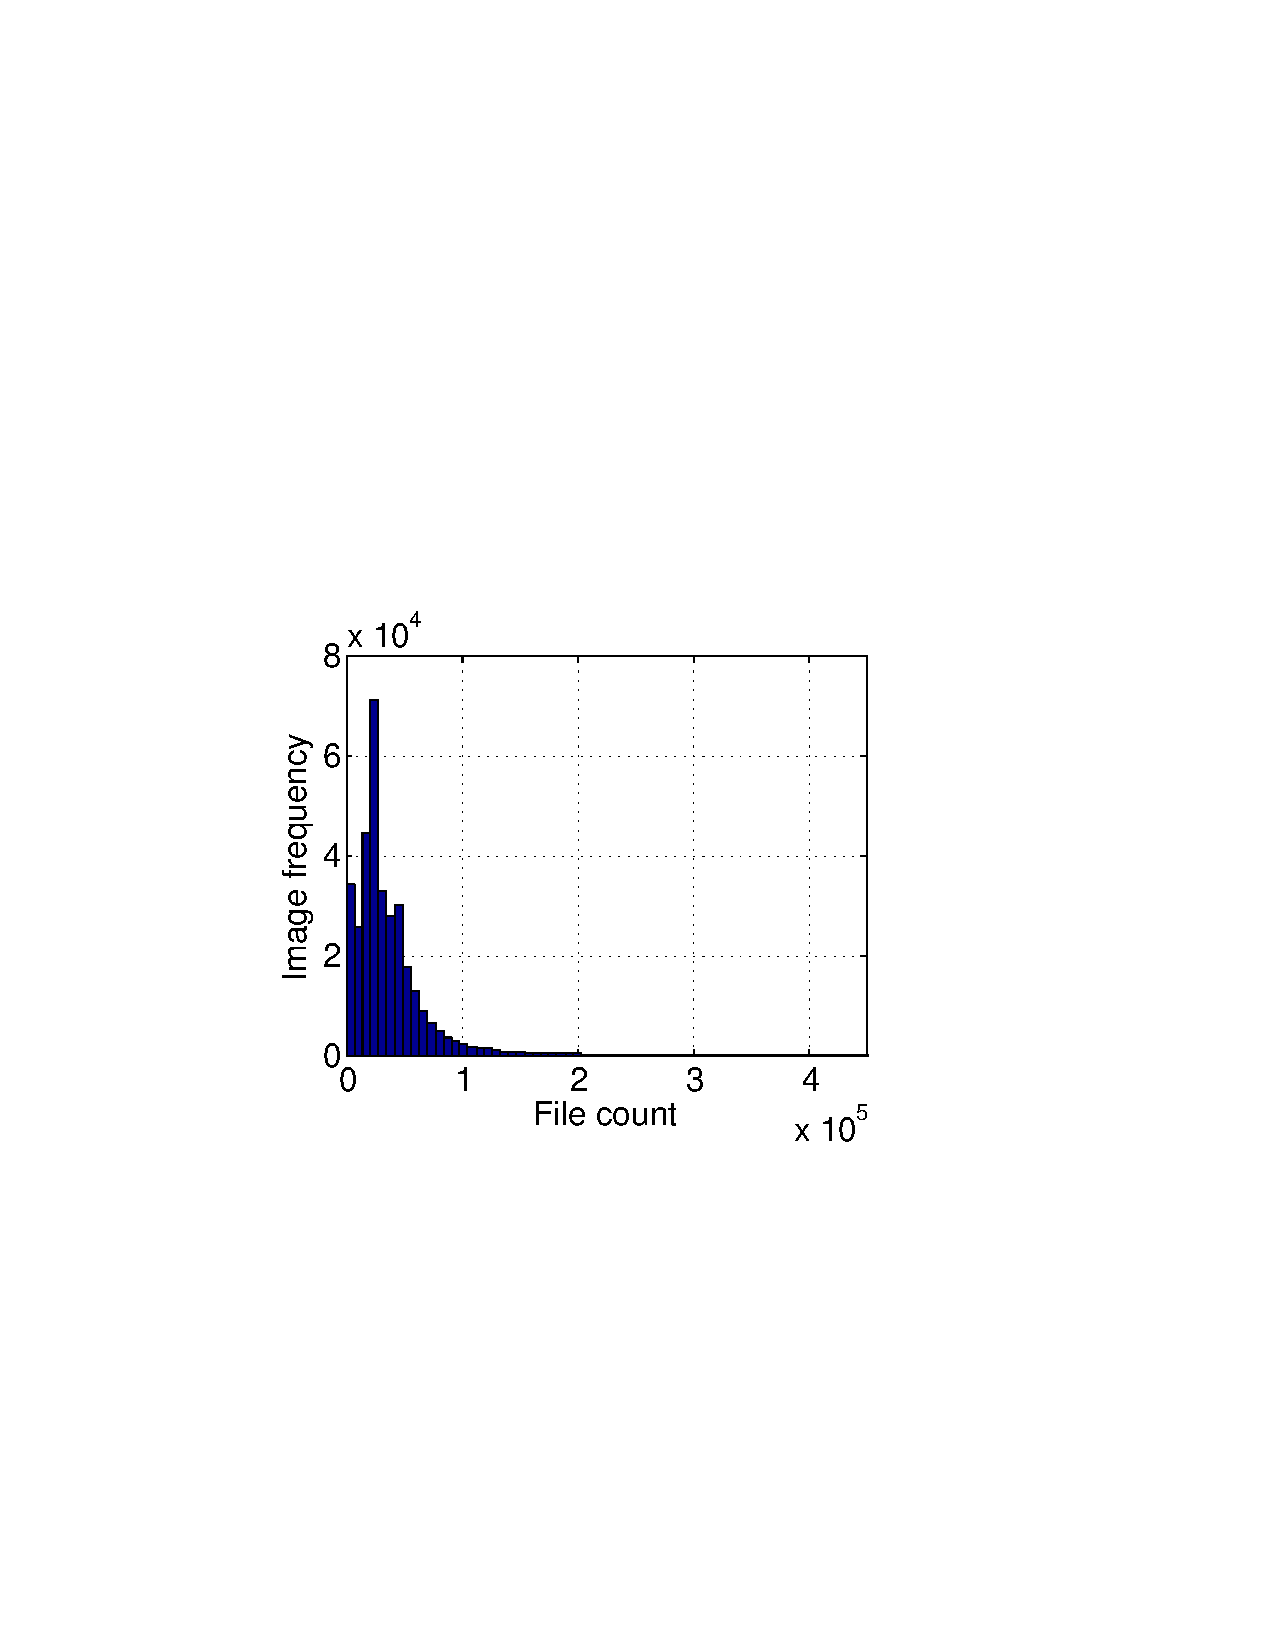
\includegraphics[width=0.21\textwidth]{graphs/image-file-cnt-pdf.pdf}%
	}
	\subfigure[Histogram of directory count per layer]{\label{fig_reference_cnt_pdf}
		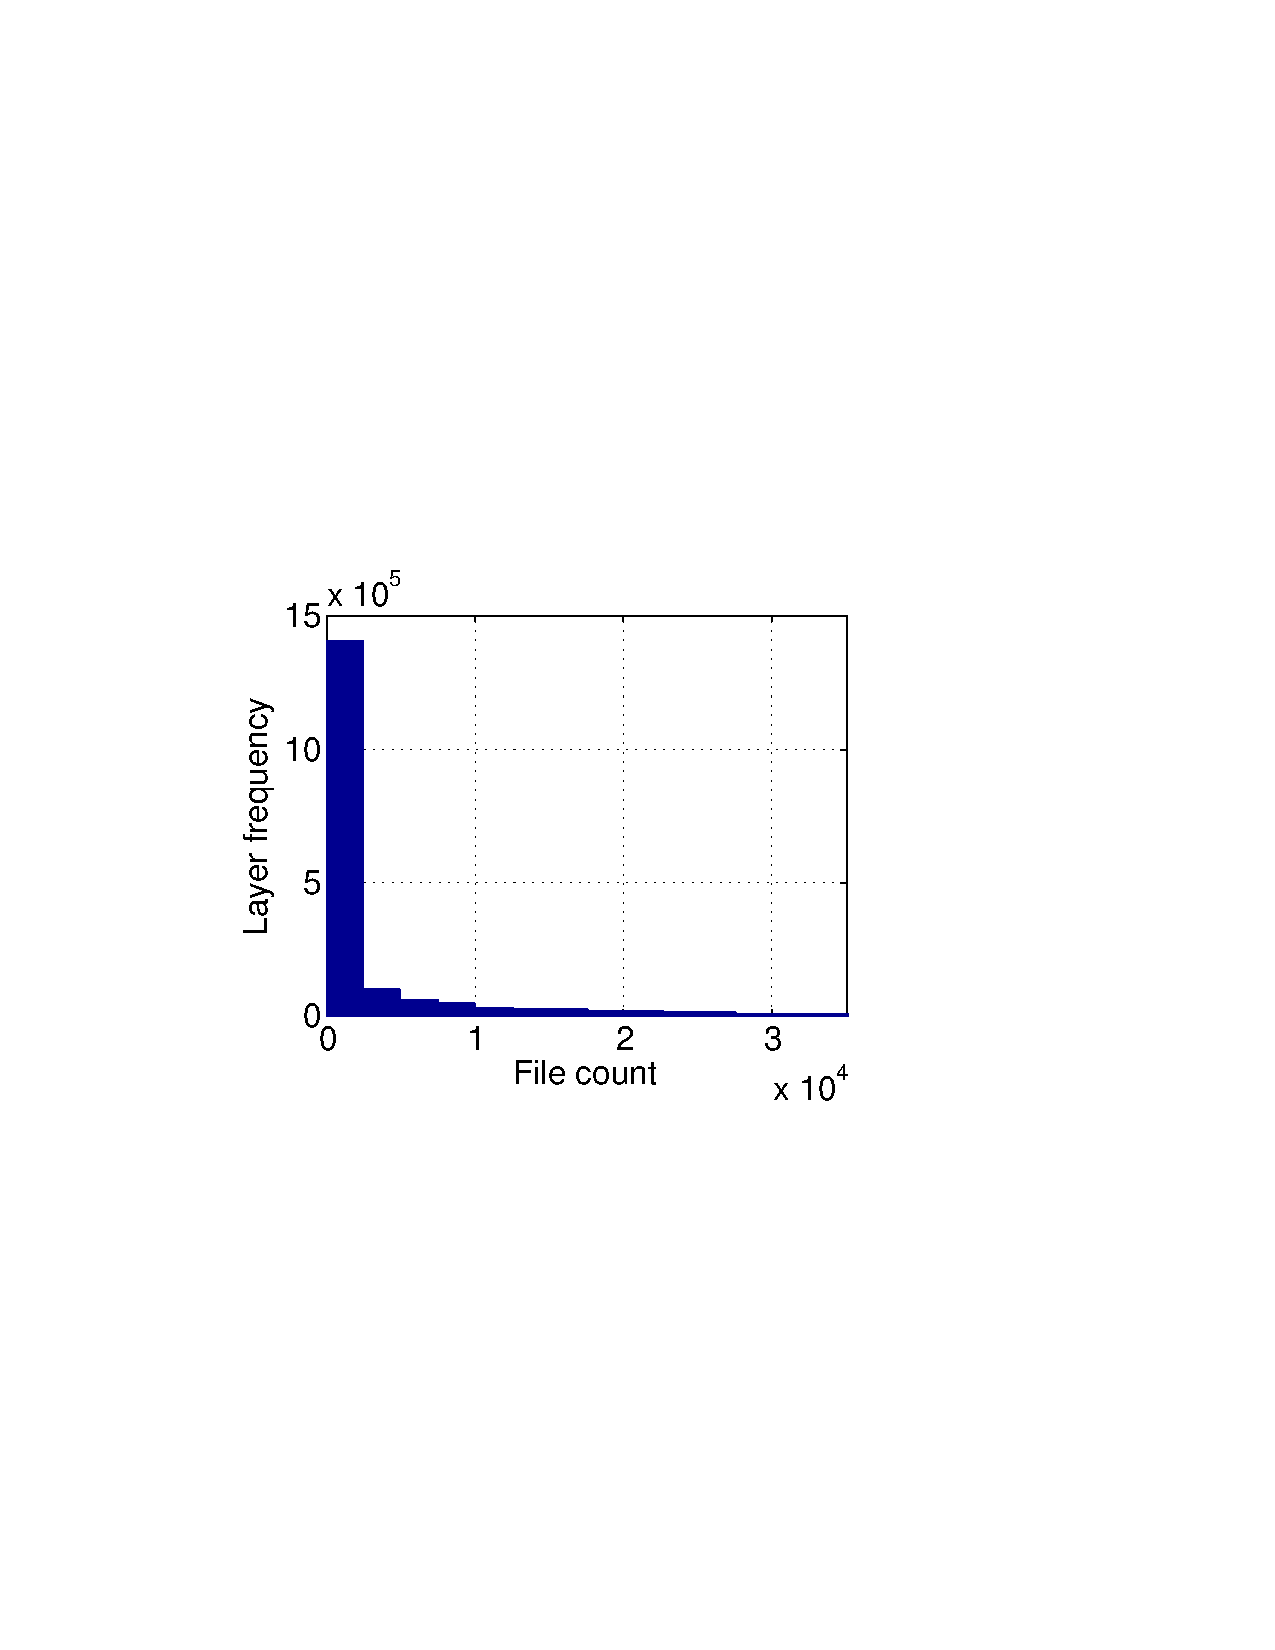
\includegraphics[width=0.22\textwidth]{graphs/layer-file-cnt-pdf.pdf}
	}
	\caption{Histogram of directory count distribution}
	\label{fig:reference-cnt}
\end{figure}

Next, we look at file and directory metrics in layers.
Figure~\ref{fig_file_cnt} and~\ref{fig_dir_cnt} show the CDFs of file
and directory counts in all layers, respectively.
%
The results show that 90\% of layers contain less than 7,410 files while half
of the layers have less than 30 files.
%
We also found that 27\% of the layers only have a single file while 7\% even showed
no files at all. We currently do not know the exact reason for the layers without files,
but one theory is that these layers use Docker volumes to store
all requred files (including executables).
% plan to investigate their corresponding images in the future.
%\nancomment{The layers are not empty since it could have directories}.
On the other hand,
the largest layer contains 826,196 files and was part of a Debian image.
%
%The average is 2,200.
%
For directories, 90\% of the layers have less than 826 directories and half of the layers consist
of less than 11 directories. We again observe a wide range with a minimum of a single directory
and a maximum of 111,940. The layer with the most directories was part of
the \textit{conjurinc/developer-quiz} image.

%\paragraph{Directory depths}

%After extracting and unpacking gzip compressed layer archival files,
Besides the count, we also calculate the maximum directory depth for each layer
(Figure~\ref{fig_layer_depth}).
%
Around 90\% of all layers have a directory depth less than 10
while for 50\% of the layers, the directory depth is less than 4. 
%
The most frequent directory depth is 3 with 313,000 layers showing
this depth value (Figure~\ref{fig_hist_layer_depth}).
%
%About 313,000 layers' layer directory depth is 3, which is the peak value in
%the figure.
%
%The maximum repeat count is 444 while the median is 4. The average is ~5.

This analysis shows that the majority of layers consists only of a small number
of files and does not contain deeply nested directory hierarchies. Hence, except
a few outliers, unpacked layers do not require a large amount of metadata from the storage
system.




